\section{信号、変化、モデル化}

\subsection{時間、信号、変化率}

水槽の水位制御では、最初に得られる情報は測定記録である。時刻 $t=0,1,2,\ldots$ [s] ごとに、水位計が返した測定値 $y_m(t)$ [cm]、目標水位 $r(t)$ [cm]、ポンプへ送った指令 $u_c(t)$ [\%]、対象へ実際に入った流量 $u(t)$ [L/s]、排水量や手で加えた水のような外乱 $d(t)$ [L/s]、水位計の読みのばらつき $n(t)$ [cm] が表に並ぶ。モータの角度、部屋の温度、移動ロボットの横ずれでも、時刻、測定された量、目標、入力指令、外乱、ノイズを同じ形式で記録できる。

制御工学では、この記録から次の値を予測し、望む動きになるように入力を選ぶ。したがって最初に必要なのは、時刻ごとに値をもつ量を一つの対象として扱い、その量の単位、変化率、入力、出力、状態との関係を区別することである。

\begin{definition}[信号]
時刻 $t$ の各値に対して数、ベクトル、または行列を対応させるものを信号という。水位 $h(t)$、温度 $T(t)$、角度 $\theta(t)$、電圧 $v(t)$、位置 $p(t)\in\R^3$ はすべて信号である。
\end{definition}

実験の記録は通常、一定のサンプリング間隔で並んだ数列である。その並びを理想化して、任意の時刻 $t$ で値が決まる関数として扱う。制御では、センサが信号を測り、制御器が信号を計算し、アクチュエータが信号を対象へ加える。

単位は式の意味を守る。角度 $\theta$ の単位を rad、時刻 $t$ の単位を s とすれば、角速度は rad/s でなければならない。したがって
\begin{equation}
  \omega(t)=\frac{\dd \theta(t)}{\dd t}
  \label{eq:angular-speed-definition}
\end{equation}
は「角度の時間変化率」として自然である。逆に、角速度を時間で積み上げれば角度に戻る。

\begin{formula}[微分と積分の対応]
初期角度 $\theta(0)$ と角速度 $\omega(t)$ が分かっているとき、角度は
\begin{equation}
  \theta(t)=\theta(0)+\int_0^t \omega(\tau)\,\dd \tau
  \label{eq:integral-angle}
\end{equation}
で与えられる。
\end{formula}

\begin{derivation}
\weq{angular-speed-definition} より
\begin{equation}
  \frac{\dd\theta}{\dd t}=\omega(t)
\end{equation}
である。両辺に $\dd t$ を掛ける記法で考えると
\begin{equation}
  \dd\theta=\omega(t)\,\dd t
\end{equation}
となる。時刻 $0$ から $t$ まで足し合わせるので
\begin{equation}
  \int_{\theta(0)}^{\theta(t)}\dd\theta
  =\int_0^t\omega(\tau)\,\dd\tau
\end{equation}
である。左辺は $\theta(t)-\theta(0)$ だから
\begin{equation}
  \theta(t)-\theta(0)=\int_0^t\omega(\tau)\,\dd\tau
\end{equation}
となり、移項して \weq{integral-angle} を得る。
\end{derivation}

\subsubsection{指数関数解の導出}

温度差、速度誤差、電気回路の電流のように「現在大きいほど速く減る」量は多い。このとき最小のモデルは
\begin{equation}
  \dot{x}(t)=-a x(t),\qquad a>0
  \label{eq:basic-decay-ode}
\end{equation}
である。ここで点は時間微分を表す。

\begin{theorem}[一次の同次線形微分方程式の解]
\weq{basic-decay-ode} の解は
\begin{equation}
  x(t)=x(0)e^{-at}
  \label{eq:basic-decay-solution}
\end{equation}
である。
\end{theorem}

\begin{derivation}
$x(t)\ne0$ の区間で両辺を $x(t)$ で割ると
\begin{equation}
  \frac{\dot{x}(t)}{x(t)}=-a
\end{equation}
である。合成関数の微分公式より、$\log |x(t)|$ の微分は
\begin{equation}
  \frac{\dd}{\dd t}\log |x(t)|=\frac{\dot{x}(t)}{x(t)}
\end{equation}
である。したがって
\begin{equation}
  \frac{\dd}{\dd t}\log |x(t)|=-a
\end{equation}
となる。時刻 $0$ から $t$ まで積分して
\begin{align}
  \int_0^t\frac{\dd}{\dd \tau}\log |x(\tau)|\,\dd\tau
  &=\int_0^t -a\,\dd\tau,\\
  \log |x(t)|-\log |x(0)|&=-at.
\end{align}
対数の性質 $\log A-\log B=\log(A/B)$ より
\begin{equation}
  \log \left|\frac{x(t)}{x(0)}\right|=-at
\end{equation}
である。両辺の指数をとれば
\begin{equation}
  \left|\frac{x(t)}{x(0)}\right|=e^{-at}
\end{equation}
となる。初期値の符号は解の途中で変わらないので、符号を含めて
\begin{equation}
  x(t)=x(0)e^{-at}
\end{equation}
を得る。
\end{derivation}

この導出を見ると、指数関数は経験的に仮定する形ではない。「変化率が現在値に比例する」という仮定から、対数の微分を通って出てくる必然的な形である。

\subsubsection{一次線形微分方程式の初期値問題}

制御対象の最小モデルは、減衰だけを表す \weq{basic-decay-ode} から、入力や外乱を受ける一次線形微分方程式へ広がる。係数 $a$ [1/s] を一定、右辺の信号 $r(t)$ の単位を $x$/s として
\begin{equation}
  \dot{x}(t)+a x(t)=r(t)
  \label{eq:first-order-linear-ivp}
\end{equation}
を考える。微分方程式だけでは解は一つに決まらない。時刻 $0$ の値
\begin{equation}
  x(0)=x_0
  \label{eq:first-order-linear-initial}
\end{equation}
を合わせて指定したものを初期値問題という。初期値は、コンデンサに最初から蓄えられている電荷、物体の初期温度、台車の初期位置や速度のように、入力を加える前から対象の内部に残っている情報を表す。

\begin{theorem}[一次線形微分方程式の積分因子解]
$a$ を定数、$r(t)$ を区分的に連続な信号とする。\weq{first-order-linear-ivp} と \weq{first-order-linear-initial} の解は
\begin{equation}
  x(t)=e^{-at}x_0+\int_0^t e^{-a(t-\tau)}r(\tau)\,\dd\tau
  \label{eq:first-order-integrating-factor-solution}
\end{equation}
である。
\end{theorem}

\begin{derivation}
\weq{first-order-linear-ivp} の両辺に $e^{at}$ を掛ける。
\begin{equation}
  e^{at}\dot{x}(t)+a e^{at}x(t)=e^{at}r(t)
\end{equation}
左辺は積の微分公式により
\begin{equation}
  \frac{\dd}{\dd t}\{e^{at}x(t)\}=e^{at}\dot{x}(t)+a e^{at}x(t)
\end{equation}
である。したがって
\begin{equation}
  \frac{\dd}{\dd t}\{e^{at}x(t)\}=e^{at}r(t)
\end{equation}
を得る。ここで $e^{at}$ を積分因子という。時刻 $0$ から $t$ まで積分すると
\begin{align}
  e^{at}x(t)-x(0)&=\int_0^t e^{a\tau}r(\tau)\,\dd\tau,\\
  x(t)&=e^{-at}x_0+\int_0^t e^{-a(t-\tau)}r(\tau)\,\dd\tau
\end{align}
となる。
\end{derivation}

\weq{first-order-integrating-factor-solution} の第一項は初期値から生じる応答であり、入力を 0 とした同次方程式
\begin{equation}
  \dot{x}+a x=0
\end{equation}
の解である。この応答を自然応答または自由応答という。特性方程式は $s+a=0$ であり、根 $s=-a$ に対応する固有モードは $e^{-at}$ である。したがって一次系の固有応答は指数関数一つで決まる。第二項は右辺信号 $r(t)$ によって作られる応答であり、強制応答という。線形方程式では、全応答は
\begin{equation}
  x(t)=x_{\mathrm{free}}(t)+x_{\mathrm{forced}}(t)
\end{equation}
のように、同次解と特殊解の和として表される。

右辺が一定値 $r(t)=r_0$ の場合は、特殊解を定数 $x_p$ として求められる。$\dot{x}_p=0$ を \weq{first-order-linear-ivp} に代入すると
\begin{equation}
  a x_p=r_0,\qquad x_p=\frac{r_0}{a}
  \label{eq:first-order-particular-constant}
\end{equation}
である。ただし $a\ne0$ とする。偏差 $z=x-x_p$ を置くと
\begin{equation}
  \dot{z}=\dot{x},\qquad
  \dot{z}+a z=0
\end{equation}
となる。変数分離法により
\begin{equation}
  \frac{\dot{z}}{z}=-a
\end{equation}
を積分して
\begin{equation}
  z(t)=z(0)e^{-at}
\end{equation}
を得る。したがって
\begin{equation}
  x(t)=\frac{r_0}{a}+
  \left(x_0-\frac{r_0}{a}\right)e^{-at}
  \label{eq:first-order-constant-input-solution}
\end{equation}
である。この式では $r_0/a$ が特殊解、括弧内の係数をもつ指数項が同次解である。

\begin{definition}[時定数]
$a>0$ の一次安定系では
\begin{equation}
  \tau=\frac{1}{a}
\end{equation}
を時定数という。時定数の単位は s であり、偏差 $z(t)$ は
\begin{equation}
  z(\tau)=z(0)e^{-1}\simeq0.368z(0)
\end{equation}
まで小さくなる。
\end{definition}

時定数は「何秒で完全に定常値へ到達するか」ではなく、偏差が同じ比率で減る速さを表す量である。$t=2\tau$ では $e^{-2}\simeq0.135$、$t=3\tau$ では $e^{-3}\simeq0.050$ になる。制御設計で応答を速くするとは、多くの場合、閉ループ方程式の係数を変えて固有モードの時定数を小さくすることを意味する。

\begin{example}[比例制御された一次対象の初期値応答]
一次対象
\begin{equation}
  \tau_p\dot{y}(t)+y(t)=K_0u(t),\qquad \tau_p>0
\end{equation}
を、比例制御器
\begin{equation}
  u(t)=k_c\{r(t)-y(t)\}
\end{equation}
で制御する。ここで $y$ は出力、$u$ は入力、$r$ は参照信号、$K_0$ は対象の静的ゲイン、$k_c$ は比例ゲインである。参照信号を一定値 $r(t)=r_0$ とすると
\begin{align}
  \tau_p\dot{y}+y&=K_0k_c(r_0-y),\\
  \tau_p\dot{y}+(1+K_0k_c)y&=K_0k_c r_0.
\end{align}
$1+K_0k_c>0$ のとき閉ループは一次安定系であり、
\begin{equation}
  a_{\mathrm{cl}}=\frac{1+K_0k_c}{\tau_p},
  \qquad
  r_{\mathrm{cl}}=\frac{K_0k_c}{\tau_p}r_0
\end{equation}
と置けば $\dot{y}+a_{\mathrm{cl}}y=r_{\mathrm{cl}}$ である。定常値と時定数は
\begin{equation}
  y_\infty=\frac{K_0k_c}{1+K_0k_c}r_0,
  \qquad
  \tau_{\mathrm{cl}}=\frac{1}{a_{\mathrm{cl}}}
  =\frac{\tau_p}{1+K_0k_c}
\end{equation}
となる。初期値を $y(0)=y_0$ とすれば
\begin{equation}
  y(t)=y_\infty+(y_0-y_\infty)e^{-t/\tau_{\mathrm{cl}}}
  \label{eq:proportional-first-order-response}
\end{equation}
である。\weq{proportional-first-order-response} の指数項は閉ループの自然応答であり、$y_\infty$ は一定参照信号に対する強制応答である。比例ゲイン $k_c$ を大きくすると $\tau_{\mathrm{cl}}$ は小さくなるが、定常値は一般に $r_0$ と一致しない。この残りの偏差を消すには、後で扱う積分動作やフィードフォワードの設計が必要になる。
\end{example}

\subsubsection{二次微分方程式への接続}

機械系では、一つの状態だけでは未来を決められないことが多い。質量ばねダンパ系の変位 $q(t)$ は、入力力 $u(t)$ と外力外乱を無視すれば
\begin{equation}
  M\ddot{q}(t)+c\dot{q}(t)+kq(t)=u(t)
  \label{eq:second-order-ode-connection}
\end{equation}
のような二次微分方程式に従う。$M$ [kg]、$c$ [N\,s/m]、$k$ [N/m] は正のパラメータである。一定入力 $u(t)=u_0$ に対する特殊解は
\begin{equation}
  q_p=\frac{u_0}{k}
\end{equation}
であり、偏差 $z=q-q_p$ は
\begin{equation}
  M\ddot{z}+c\dot{z}+kz=0
\end{equation}
を満たす。指数関数形 $z=e^{st}$ を代入すると
\begin{equation}
  Ms^2+cs+k=0
  \label{eq:mass-spring-characteristic}
\end{equation}
を得る。\weq{mass-spring-characteristic} が二次系の特性方程式であり、その二つの根が固有モードを決める。根が相異なる実数 $s_1,s_2$ なら固有応答は
\begin{equation}
  z(t)=C_1e^{s_1t}+C_2e^{s_2t}
\end{equation}
であり、複素共役根なら減衰振動として表される。係数 $C_1,C_2$ は、初期変位 $q(0)$ と初期速度 $\dot{q}(0)$ の二つの初期値から決まる。

この二次方程式も、状態を
\begin{equation}
  x(t)=\begin{bmatrix}q(t)\\ \dot{q}(t)\end{bmatrix}
\end{equation}
と選べば一階の連立微分方程式になる。つまり一次系で見た同次解、特殊解、初期値、時定数、固有応答という考えは、二次系では「固有根が一つから二つへ増える」形で拡張される。後の章で扱う行列指数関数は、この連立一次系の自然応答をまとめて書くための記法である。

\subsubsection{テイラー展開による局所近似}

制御器が利用できる情報は、現在値、過去の測定値、既知の入力に限られる。それでも、現在の値と変化率が分かれば、短い時間後の値は近似できる。

\begin{theorem}[テイラーの定理の一次近似]
十分なめらかな関数 $x(t)$ について、$\Delta t$ が小さいとき
\begin{equation}
  x(t+\Delta t)=x(t)+\dot{x}(t)\Delta t+O(\Delta t^2)
\end{equation}
である。二次まで残すと
\begin{equation}
  x(t+\Delta t)=x(t)+\dot{x}(t)\Delta t+
  \frac{1}{2}\ddot{x}(t)\Delta t^2+O(\Delta t^3)
\end{equation}
である。
\end{theorem}

\begin{derivation}
テイラーの定理より、$t$ のまわりの展開は
\begin{equation}
  x(t+\Delta t)=x(t)+x'(t)\Delta t+
  \frac{x''(t)}{2!}\Delta t^2+
  \frac{x^{(3)}(t)}{3!}\Delta t^3+\cdots
\end{equation}
である。ここで $x'(t)=\dot{x}(t)$、$x''(t)=\ddot{x}(t)$ と書き直す。一次近似では $\Delta t^2$ 以上の項をまとめて $O(\Delta t^2)$ と書くので、最初の式を得る。二次近似では $\Delta t^3$ 以上の項をまとめるので、二つ目の式を得る。
\end{derivation}

この定理は、線形化、数値積分、離散化の土台になる。小さい $\Delta t$ では $\Delta t^2$ や $\Delta t^3$ はさらに小さくなるため、短い時間だけなら最初の数項で動きを近似できる。

\subsubsection{陽的 Euler 法による数値積分と刻み幅}

連続時間モデル
\begin{equation}
  \dot{x}(t)=f(x(t),u(t),d(t),p,t)
  \label{eq:continuous-state-model-for-integration}
\end{equation}
は、各時刻における状態の変化率を与える。計算機シミュレーションでは、連続なすべての時刻をそのまま扱わず、時刻列
\begin{equation}
  t_k=t_0+kh,\qquad k=0,1,2,\ldots
\end{equation}
上の近似値 $x_k\simeq x(t_k)$ を順に更新する。ここで $h>0$ は刻み幅またはシミュレーションステップサイズであり、単位は s である。$x_i$ の単位が温度 K、電圧 V、位置 m のいずれであっても、$f_i$ の単位は $x_i$/s でなければならない。したがって $h f_i$ は $x_i$ と同じ単位をもち、状態更新で足し合わせられる量になる。

\begin{formula}[陽的 Euler 法]
\weq{continuous-state-model-for-integration} において、区間 $[t_k,t_{k+1})$ で入力と外乱を代表値 $u_k$、$d_k$ により近似する。$f$ が十分なめらかで、刻み幅 $h$ が小さいとき、陽的 Euler 法は
\begin{equation}
  x_{k+1}=x_k+h f(x_k,u_k,d_k,p,t_k)
  \label{eq:explicit-euler-state-update}
\end{equation}
により状態を更新する。
\end{formula}

\begin{derivation}
微分方程式を時刻 $t_k$ から $t_{k+1}=t_k+h$ まで積分すると、厳密解は
\begin{equation}
  x(t_{k+1})=x(t_k)+
  \int_{t_k}^{t_k+h} f(x(\tau),u(\tau),d(\tau),p,\tau)\,\dd\tau
  \label{eq:exact-integral-state-update}
\end{equation}
を満たす。陽的 Euler 法では、この積分区間の被積分関数を左端の値
\begin{equation}
  f(x(t_k),u_k,d_k,p,t_k)
\end{equation}
で一定と近似する。すると
\begin{align}
  x(t_{k+1})
  &\simeq x(t_k)+
  \int_{t_k}^{t_k+h} f(x(t_k),u_k,d_k,p,t_k)\,\dd\tau\\
  &=x(t_k)+h f(x(t_k),u_k,d_k,p,t_k)
\end{align}
となる。厳密値 $x(t_k)$ の代わりに近似値 $x_k$ を使うと \weq{explicit-euler-state-update} を得る。
\end{derivation}

この更新式は、微分を差分で置き換えただけの記法ではなく、現在の変化率を時間 $h$ だけ積み上げる近似である。一回の更新を厳密値 $x(t_k)$ から開始した場合、テイラー展開により
\begin{align}
  x(t_k+h)
  &=x(t_k)+h\dot{x}(t_k)+\frac{h^2}{2}\ddot{x}(\xi_k)\\
  &=x(t_k)+h f(x(t_k),u_k,d_k,p,t_k)+O(h^2)
\end{align}
と書ける。ただし $\xi_k$ は $t_k$ と $t_k+h$ の間の時刻であり、区間内で入力と外乱を一定値で近似しているとする。したがって一ステップの局所離散化誤差は $O(h^2)$ である。一方、固定した時間区間 $[t_0,T]$ を $N=(T-t_0)/h$ ステップで進むと、局所誤差が各ステップで蓄積する。$f$ が状態に関して Lipschitz 連続で、必要な導関数が有界であるなら、陽的 Euler 法の大域誤差は $O(h)$ で抑えられる。刻み幅を半分にすると、同じ時間区間のステップ数はほぼ二倍になり、大域誤差は一次の精度で小さくなる。

刻み幅は精度だけでなく数値安定性にも関わる。最も単純な減衰方程式
\begin{equation}
  \dot{z}(t)=-a z(t),\qquad a>0
\end{equation}
に陽的 Euler 法を適用すると
\begin{equation}
  z_{k+1}=(1-ah)z_k
  \label{eq:euler-stability-test}
\end{equation}
である。連続時間では任意の $a>0$ で $z(t)$ は 0 へ減衰する。しかし離散更新では
\begin{equation}
  |1-ah|<1
\end{equation}
すなわち
\begin{equation}
  0<h<\frac{2}{a}
  \label{eq:euler-stability-step-bound}
\end{equation}
でなければ、数列 $z_k$ は減衰しない。$h$ が大きすぎると、連続時間モデルは安定であるにもかかわらず、数値解だけが符号反転を伴って増大することがある。これは対象の物理的な不安定性ではなく、数値積分法と刻み幅の組合せから生じる数値不安定性である。

RC 回路
\begin{equation}
  C_e\dot{v}_C(t)=\frac{u(t)-v_C(t)}{R}
\end{equation}
で、抵抗 $R$ [$\Omega$]、容量 $C_e$ [F] を一定、入力電圧を区間ごとに $u_k$ [V] で一定と仮定する。時定数を
\begin{equation}
  \tau=R C_e
\end{equation}
と置くと、状態 $x=v_C$ は
\begin{equation}
  \dot{x}(t)=-\frac{1}{\tau}x(t)+\frac{1}{\tau}u(t)
\end{equation}
に従う。陽的 Euler 法では
\begin{align}
  x_{k+1}
  &=x_k+h\left(-\frac{1}{\tau}x_k+\frac{1}{\tau}u_k\right)\\
  &=\left(1-\frac{h}{\tau}\right)x_k+\frac{h}{\tau}u_k
  \label{eq:rc-explicit-euler-update}
\end{align}
である。比 $h/\tau$ は無次元であり、電圧 $x_k$ と $u_k$ に掛けられる係数として解釈できる。入力を 0 とした自然応答では、数値的な減衰条件は
\begin{equation}
  0<h<2\tau
\end{equation}
である。たとえば $\tau=0.5\,\mathrm{s}$ なら $h=0.01\,\mathrm{s}$ は時定数に比べて十分小さいが、$h=1.5\,\mathrm{s}$ は \weq{euler-stability-step-bound} を破り、連続時間の RC 回路とは異なる発散的な数列を作る。後の状態空間離散化や実装章で扱うサンプリング周期は、この刻み幅を制御器、センサ、アクチュエータ、数値積分法の条件と合わせて選ぶ問題である。

\subsection{入力、出力、状態}

部屋の温度制御では、温度センサの測定値 $y_m(t)$、目標温度 $r(t)$、ヒータ指令 $u_c(t)$、外気温や窓の開閉による外乱 $d(t)$ が時刻ごとに記録される。しかし、同じ時刻に $y_m(t)=24.8\,^\circ\mathrm{C}$、$r(t)=25\,^\circ\mathrm{C}$、同じヒータ指令であっても、壁や家具に蓄えられた熱、ヒータ素子の温度、空気の混ざり方が異なれば、次の 1 分の温度変化は一致しない。モータでも、同じ角度を測っていても角速度が正か負かで次の角度は変わる。水槽でも、同じ水位であっても流入弁や排水の状態が異なれば次の水位は変わる。

このため、測定された出力だけでは、次時刻の値を決める情報として不十分である。対象へ意図して加える量、対象から評価する量、意図せず入る作用、測定に混じる誤差、未来の変化を決める内部情報を分けて書く必要がある。

\begin{definition}[信号の役割]
時間信号のうち、制御対象へ意図して加える作用を入力 $u$、制御対象から取り出して評価または制御に使う量を出力 $y$、制御器が選ばないのに対象へ作用する量を外乱 $d$、測定やモデル化に混じる誤差成分をノイズ $n$ という。目標として与える信号を参照信号 $r$、制御器がアクチュエータへ渡す信号をアクチュエータ指令 $u_c$、センサが実際に返す信号をセンサ測定値 $y_m$ と呼ぶ。
\end{definition}

\begin{definition}[パラメータ、測定量、状態]
モデルの係数として扱い、通常は時間積分しない定数またはゆっくり変わる量をパラメータ $p$ という。抵抗 $R$、容量 $C$、質量 $M$、ばね定数 $k$、粘性係数 $c$、慣性モーメント $J$ は典型的なパラメータであり、それぞれ固有の単位をもつ。センサが観測しようとしている物理量を測定量といい、測定量にノイズ、バイアス、量子化、較正誤差が加わって制御器へ届いた信号をセンサ測定値という。現在の値と今後の入力が分かれば以後の変化を計算するのに十分な量の組を状態 $x$ という。
\end{definition}

同じ時間関数でも、役割が違えば制御上の扱いは変わる。参照信号 $r(t)$ は「こう動いてほしい」という外から与えた希望であり、出力 $y(t)$ は対象が実際に示す量である。温度制御で目標温度 $r(t)=25\,^\circ\mathrm{C}$ を与えても、部屋の温度 $y(t)$ がすぐ $25\,^\circ\mathrm{C}$ になるわけではない。制御器は誤差
\begin{equation}
  e(t)=r(t)-y_m(t)
  \label{eq:feedback-error-signal}
\end{equation}
を使ってアクチュエータ指令 $u_c(t)$ を計算する。アクチュエータには飽和、遅れ、変換係数があるため、対象に実際に入る入力 $u(t)$ はしばしば $u_c(t)$ と一致しない。たとえば PWM デューティ比 $u_c$ からヒータ電力 $u$ が作られる場合、$u_c$ は無次元、$u$ は W である。

以後しばらくは、連続時間 $t$ の単位を s とし、集中定数モデルを扱う。集中定数モデルとは、温度、電圧、位置のような代表値だけで対象を表し、空間分布や波動伝搬を明示しない近似である。信号は必要な範囲で区分的に連続、パラメータは特に断らない限り一定、センサノイズは測定値へ加法的に入るものと仮定する。この仮定により、まず
\begin{align}
  \dot{x}(t)&=f(x(t),u(t),d(t),p,t),\label{eq:plant-signal-model}\\
  y(t)&=g(x(t),u(t),d(t),p,t),\\
  y_m(t)&=y(t)+n(t),\\
  u(t)&=\phi_a(u_c(t),p_a,t)
\end{align}
という形で信号の入出力関係を整理できる。$x$ は状態、$u$ は対象へ入る実入力、$d$ は外乱、$p$ は対象のパラメータ、$p_a$ はアクチュエータのパラメータである。$y$ はモデル上の出力または制御量、$y_m$ はセンサ測定値であり、$n$ は $y$ と同じ単位をもつ測定ノイズとして書いている。ノイズを確率過程として平均や分散で扱うのは後の推定の章で行うが、ここでは「測定値が真値そのものではない」という区別が重要である。

外乱とノイズは、制御系へ入る位置が異なるため、モデル内で区別して扱う。外乱 $d$ は対象の運動方程式や保存則に入り、状態そのものを変化させる。ノイズ $n$ は主にセンサ測定値に入り、状態が同じであっても制御器に入力される値を変える。風が台車を押す作用は外乱であり、位置センサの読みのちらつきはノイズである。両者を同じ「誤差」と呼ぶと、フィードバックで抑制すべきずれ、推定で平均化すべきずれ、モデルに作用として入れるべき成分を混同する。

線形時不変近似では、\weq{plant-signal-model} は
\begin{align}
  \dot{x}(t)&=Ax(t)+Bu(t)+Ed(t),\label{eq:lti-disturbance-model}\\
  y(t)&=Cx(t)+D_u u(t)+D_d d(t),\\
  y_m(t)&=y(t)+n(t)
\end{align}
と書ける。行列 $A$ は状態が自然にどう変わるか、$B$ は入力が状態へどう入るか、$E$ は外乱が状態へどう入るかを表す。$C$ は状態から出力を取り出す行列であり、$D_u$ と $D_d$ は入力や外乱が状態を経ずに出力へ直接現れる成分である。この形は後で扱う状態空間表現そのものであり、フィードバックでは $r-y_m$ から入力を作り、推定では $u$ と $y_m$ から見えない状態 $x$ を推定する。

同じ記号が時間関数として並んでいても、対象へ作用して状態を変える信号、センサで混じる信号、内部に蓄えられる量は同じ場所に入らない。この入る位置を先に固定しないと、外乱を制御器の入力として扱ったり、ノイズを物理状態の変化として扱ったりする誤りが生じる。図\ref{fig:signal-modeling-examples} は、熱系を例にして信号の役割、平衡点からの偏差、局所線形化、陽的 Euler 法の刻み幅を一枚に対応させたものである。

\begin{figure}[tb]
\centering
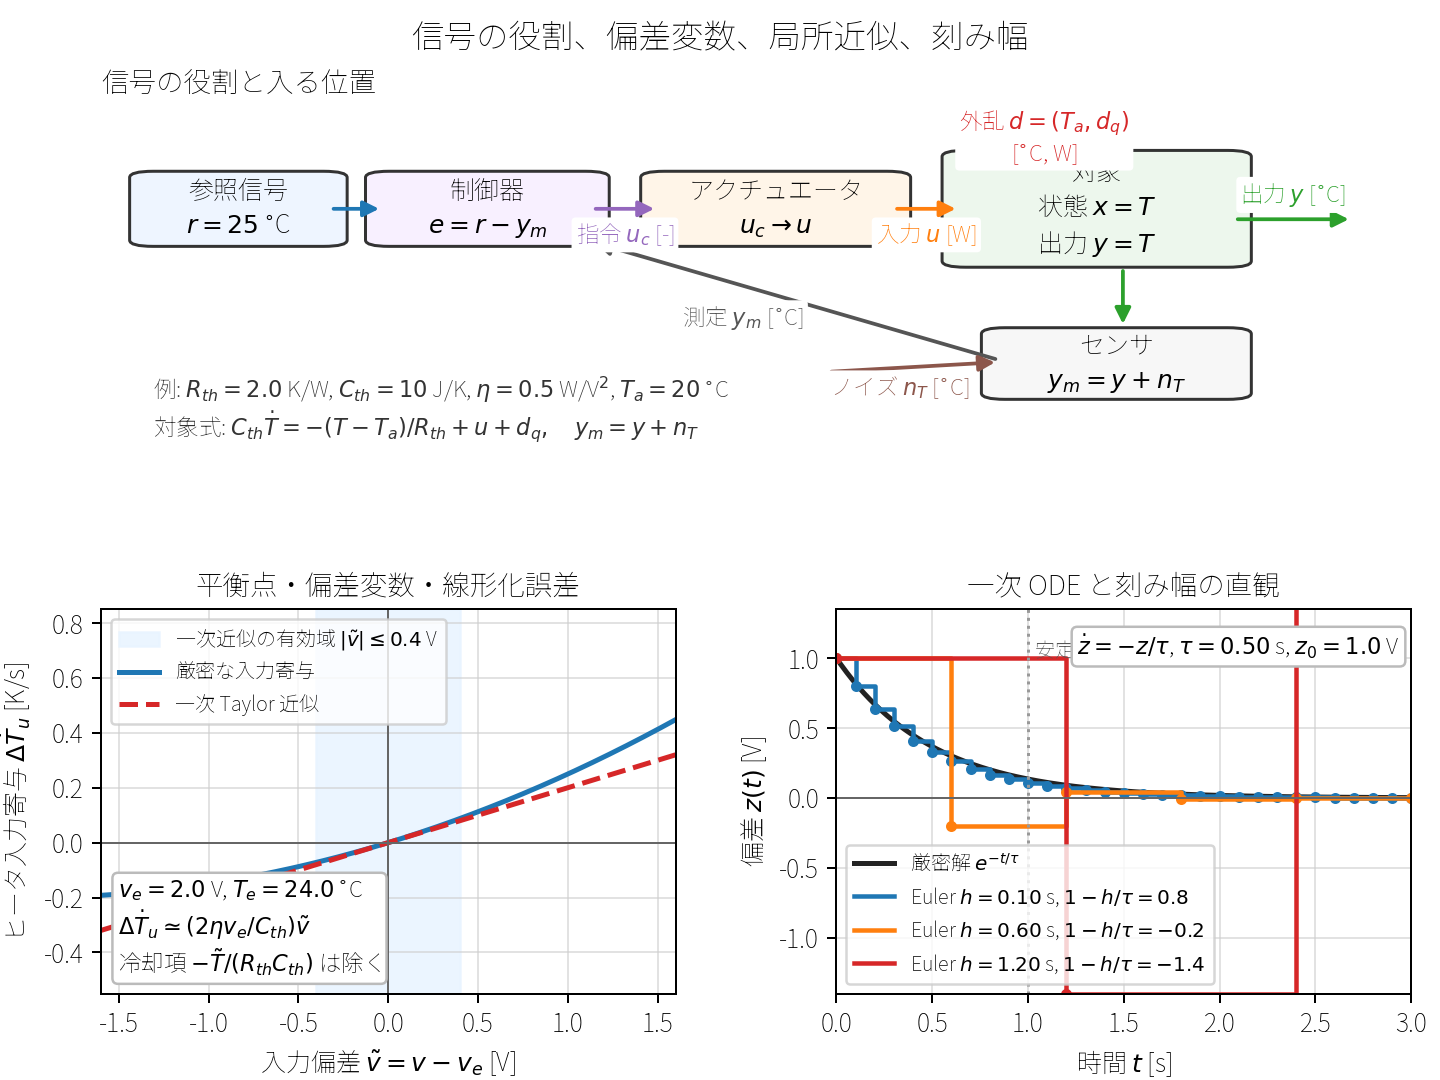
\includegraphics[width=0.96\linewidth,bb=0 0 1440 1080]{figures/signal_modeling_examples.png}
\caption{信号の役割、偏差変数、局所線形化、数値積分刻み幅の対応。上段は熱系における参照信号、入力、出力、外乱、ノイズ、状態の入る位置を示す。左下は $T_a=20\,^\circ\mathrm{C}$、$R_{\mathrm{th}}=2.0\,\mathrm{K/W}$、$C_{\mathrm{th}}=10\,\mathrm{J/K}$、$\eta=0.5\,\mathrm{W/V^2}$、$v_e=2.0\,\mathrm{V}$ の動作点で、ヒータ電圧偏差 $\tilde{v}$ が温度変化率へ与える入力寄与 $\Delta\dot{T}_u$ とその一次 Taylor 近似を比較している。完全な線形化式には、これに加えて冷却による $-\tilde{T}/(R_{\mathrm{th}}C_{\mathrm{th}})$ も入る。右下は $\dot{z}=-z/\tau$、$\tau=0.50\,\mathrm{s}$ に陽的 Euler 法を適用し、刻み幅 $h$ によって精度と数値安定性が変わることを示す。}
\label{fig:signal-modeling-examples}
\end{figure}

\begin{practice}[信号分類と局所近似の確認]
図\ref{fig:signal-modeling-examples} の上段で、対象の状態を直接変える信号と、センサ測定値だけを変える信号をそれぞれ列挙せよ。次に、左下のパラメータから平衡温度 $T_e$ を計算し、$\tilde{v}=0.4\,\mathrm{V}$ と $\tilde{v}=1.2\,\mathrm{V}$ について、温度変化率へのヒータ入力寄与
\begin{equation}
  \frac{\eta\{(v_e+\tilde{v})^2-v_e^2\}}{C_{\mathrm{th}}},
  \qquad
  \frac{2\eta v_e}{C_{\mathrm{th}}}\tilde{v}
\end{equation}
を比較せよ。この二つの量は入力項だけの比較であり、完全な $\dot{\tilde{T}}$ には冷却項 $-\tilde{T}/(R_{\mathrm{th}}C_{\mathrm{th}})$ も加わることを確認せよ。さらに右下の $\tau=0.50\,\mathrm{s}$ について、$h=0.10\,\mathrm{s}$、$0.60\,\mathrm{s}$、$1.20\,\mathrm{s}$ の更新係数 $1-h/\tau$ を求め、連続時間の安定性と数値更新の安定性が一致しない場合を説明せよ。
\end{practice}

\subsubsection{標準例における信号の役割}

熱系では、部屋または小さな物体の代表温度を $T(t)$ [$^\circ\mathrm{C}$] とし、周囲温度を $T_a(t)$ [$^\circ\mathrm{C}$]、ヒータから実際に入る熱流を $u(t)$ [W] とする。熱容量 $C_{\mathrm{th}}$ [J/K] と熱抵抗 $R_{\mathrm{th}}$ [K/W] を一定パラメータとみなすと、単純なモデルは
\begin{equation}
  C_{\mathrm{th}}\dot{T}(t)
  =-\frac{T(t)-T_a(t)}{R_{\mathrm{th}}}+u(t)+d_q(t)
  \label{eq:thermal-signal-example}
\end{equation}
である。状態は $x=T$、入力はヒータ熱流 $u$、外乱は周囲温度 $T_a$ と未知熱流 $d_q$ である。制御したい出力を $y=T$、温度センサの測定値を $y_m=T+n_T$ と置けば、参照信号 $r=T_{\mathrm{ref}}$ は目標温度である。ここで $T_a$ は測れることも測れないこともある。測れる外乱はフィードフォワード補償に使えるが、測れない外乱はフィードバックで結果として抑える。

RC 回路では、コンデンサ電圧を $v_C(t)$ [V]、入力電圧を $u(t)=v_{\mathrm{in}}(t)$ [V]、外からコンデンサ節点へ流れ込む未知電流を $d_i(t)$ [A] とする。抵抗 $R$ [$\Omega$] と容量 $C$ [F] が一定なら、キルヒホッフの電流則から
\begin{equation}
  C\dot{v}_C(t)=\frac{u(t)-v_C(t)}{R}+d_i(t)
  \label{eq:rc-signal-example}
\end{equation}
を得る。$x=v_C$ とすれば、出力は $y=v_C$、センサ測定値は $y_m=v_C+n_v$ である。$R$ や $C$ は信号ではなくパラメータとして扱うが、温度で抵抗値が変わるほど精密に見る場合は、$R(t)$ をゆっくり変化する未知パラメータまたは追加状態として推定することがある。

質量ばねダンパ系では、位置 $q(t)$ [m]、速度 $\dot{q}(t)$ [m/s]、力入力 $u(t)$ [N]、外力外乱 $d_F(t)$ [N] を使う。質量 $M$ [kg]、粘性係数 $c$ [N\,s/m]、ばね定数 $k$ [N/m] を一定とすると、ニュートンの運動方程式は
\begin{equation}
  M\ddot{q}(t)+c\dot{q}(t)+kq(t)=u(t)+d_F(t)
  \label{eq:msd-signal-example}
\end{equation}
である。状態を
\begin{equation}
  x(t)=\begin{bmatrix}q(t)\\ \dot{q}(t)\end{bmatrix}
\end{equation}
と置くと
\begin{align}
  \dot{x}(t)&=
  \begin{bmatrix}
    0&1\\
    -k/M&-c/M
  \end{bmatrix}x(t)
  +\begin{bmatrix}0\\ 1/M\end{bmatrix}u(t)
  +\begin{bmatrix}0\\ 1/M\end{bmatrix}d_F(t),\label{eq:msd-state-signal-example}\\
  y(t)&=\begin{bmatrix}1&0\end{bmatrix}x(t),\\
  y_m(t)&=y(t)+n_q(t)
\end{align}
と書ける。位置センサしかない場合、測定量は位置 $q$ であり、センサ測定値は $q+n_q$ である。速度 $\dot{q}$ は状態の一部だが直接測れていないので、未測定状態である。後でオブザーバや Kalman フィルタを導入するのは、このような未測定状態を、入力と測定値の履歴から推定するためである。

DC モータなら、端子電圧 $v(t)$ [V] は入力、角速度 $\omega(t)$ [rad/s] や角度 $\theta(t)$ [rad] は出力になりうる。負荷トルク $\tau_L(t)$ [N\,m] は、制御器が直接選んでいないので外乱である。電機子インダクタンス $L$ [H]、抵抗 $R$ [$\Omega$]、逆起電力定数 $K_e$ [V\,s/rad]、トルク定数 $K_t$ [N\,m/A]、慣性モーメント $J$ [kg\,m$^2$]、粘性係数 $b$ [N\,m\,s/rad] を一定パラメータとすると、単純化したモデルは
\begin{align}
  L\dot{i}(t)&=-R i(t)-K_e\omega(t)+v(t),\label{eq:dc-motor-current}\\
  J\dot{\omega}(t)&=K_t i(t)-b\omega(t)-\tau_L(t),\label{eq:dc-motor-speed}\\
  \dot{\theta}(t)&=\omega(t).\label{eq:dc-motor-angle}
\end{align}
となる。

DC モータの端子電圧から角度までの関係は、代数的な直接変換ではなく、電気系と機械系の状態を通る因果連鎖として表される。電圧はまず電流を変化させ、電流がトルクを発生させ、トルクが角速度を変化させ、角速度の積分として角度が変化する。この因果連鎖を式の中に残すために、状態を導入する。

DC モータでは
\begin{equation}
  x(t)=\begin{bmatrix}i(t)\\ \omega(t)\\ \theta(t)\end{bmatrix}
\end{equation}
を状態にできる。状態 $x$、入力 $u$、外乱 $d$、パラメータ $p$、出力 $y$ を使うと、多くの対象は
\begin{align}
  \dot{x}(t)&=f(x(t),u(t),d(t),p,t),\label{eq:nonlinear-state-model}\\
  y(t)&=g(x(t),u(t),d(t),p,t)
\end{align}
と書ける。$f$ は内部がどう変わるか、$g$ はどの量が出力として取り出されるかを表す。

状態と出力は同じではない。状態は未来を計算するための内部記述であり、出力は目的やセンサ配置に応じて選ぶ見え方である。DC モータで角度制御をするなら $y=\theta$ と置くことが多いが、電流 $i$ と角速度 $\omega$ も未来の角度を決めるので状態に含める。電流センサがなければ $i$ は未測定状態であり、角度エンコーダがあれば $\theta+n_\theta$ がセンサ測定値である。状態フィードバックの章では $u=-Kx+r_u$ のように状態が使える場合を扱い、推定の章では測定値から $\hat{x}$ を作って、測れない状態を補う。

\subsection{平衡点、偏差変数、線形化}

\begin{definition}[平衡点]
時間に陽に依存しない系 $\dot{x}=f(x,u)$ において、一定入力 $u_e$ と状態 $x_e$ が
\begin{equation}
  f(x_e,u_e)=0
\end{equation}
を満たすとき、$(x_e,u_e)$ を平衡点という。
\end{definition}

平衡点では状態の変化率が 0 なので、入力を $u_e$ に保てば状態は $x_e$ に留まる。熱系なら一定温度、RC 回路なら一定電圧、モータなら一定速度、水槽なら一定水位が平衡点の例である。外乱やパラメータを明示するモデル
\begin{equation}
  \dot{x}=f(x,u,d,p)
\end{equation}
では、一定外乱 $d_e$ とパラメータ $p$ を固定したうえで
\begin{equation}
  f(x_e,u_e,d_e,p)=0
\end{equation}
を満たす組を平衡点として扱う。周囲温度や負荷トルクが変われば、同じ入力でも平衡点は変わりうる。時間に陽に依存するモデルや周期的に動く基準運動では、厳密には一点の平衡点ではなく基準軌道のまわりで偏差を考えるが、本節ではまず一定値に留まる動作点を扱う。

\begin{definition}[偏差変数]
制御では絶対値より平衡点からのずれを見る。そこで
\begin{equation}
  \tilde{x}=x-x_e,
  \qquad
  \tilde{u}=u-u_e
  \label{eq:deviation-definition}
\end{equation}
を偏差変数という。すると $x=x_e+\tilde{x}$、$u=u_e+\tilde{u}$ である。
\end{definition}

偏差変数は無次元の誤差ではない。$x_i$ が温度なら $\tilde{x}_i$ も温度差の単位 K をもち、$u_j$ が力なら $\tilde{u}_j$ も N をもつ。必要なら後で基準値や許容幅で割って無次元化するが、線形化そのものでは物理単位を保ったまま計算する。平衡点は定数なので $\dot{x}_e=0$ であり、
\begin{equation}
  \dot{\tilde{x}}=\frac{\dd}{\dd t}(x-x_e)=\dot{x}
\end{equation}
である。出力も同じ考えで、$y_e=g(x_e,u_e)$ と置けば $\tilde{y}=y-y_e$ を出力偏差として使える。

\begin{definition}[ヤコビアン]
ベクトル値関数 $f(x,u)\in\R^n$ の各成分を各変数で偏微分して並べた行列をヤコビアンという。$x\in\R^n$、$u\in\R^m$ なら
\begin{equation}
  \frac{\pp f}{\pp x}=\left[\frac{\pp f_i}{\pp x_j}\right]_{i,j},
  \qquad
  \frac{\pp f}{\pp u}=\left[\frac{\pp f_i}{\pp u_j}\right]_{i,j}
\end{equation}
である。
\end{definition}

$\dot{x}=f(x,u)$ では $f_i$ の単位は $x_i$/s である。したがって $\pp f_i/\pp x_j$ の単位は $(x_i/\mathrm{s})/x_j$、$\pp f_i/\pp u_j$ の単位は $(x_i/\mathrm{s})/u_j$ になる。$A=\pp f/\pp x$ は $n\times n$ 行列、$B=\pp f/\pp u$ は $n\times m$ 行列であり、$A\tilde{x}$ と $B\tilde{u}$ の各成分はどちらも $x_i$/s の単位をもつ。状態の各成分が位置、速度、電流のように違う単位をもつとき、行列の成分も同じ単位ではない。

\begin{theorem}[一次テイラー展開による線形化]
非線形系 $\dot{x}=f(x,u)$ が平衡点 $(x_e,u_e)$ の近くで十分なめらかなら、偏差変数 $\tilde{x}$、$\tilde{u}$ は一次近似で
\begin{equation}
  \dot{\tilde{x}}=A\tilde{x}+B\tilde{u}
  \label{eq:linearized-model}
\end{equation}
に従う。ただし
\begin{equation}
  A=\left.\frac{\pp f}{\pp x}\right|_{(x_e,u_e)},
  \qquad
  B=\left.\frac{\pp f}{\pp u}\right|_{(x_e,u_e)}
\end{equation}
である。
\end{theorem}

ここで「十分なめらか」とは、少なくとも平衡点の近傍で $f$ の一次偏微分が存在して連続であり、二次の誤差項を小さくできるという意味である。より安全には $f$ が二回連続微分可能で、二階偏微分が近傍で有界であると仮定する。この仮定により、$\delta z=[\tilde{x}^\T,\tilde{u}^\T]^\T$ と置いたとき、捨てた項 $r_2(\delta z)$ は
\begin{equation}
  \lVert r_2(\delta z)\rVert \le c\lVert \delta z\rVert^2
\end{equation}
を満たす定数 $c$ で抑えられる。したがって一次モデルは $\tilde{x}$ と $\tilde{u}$ が小さい範囲でだけ信頼できる。入力飽和、摩擦の符号切替、接触の有無のように式が滑らかでない現象をまたぐと、この線形化の仮定は崩れる。

\begin{derivation}
$x=x_e+\tilde{x}$、$u=u_e+\tilde{u}$ を $\dot{x}=f(x,u)$ に代入する。$x_e$ は定数なので $\dot{x}=\dot{\tilde{x}}$ である。したがって
\begin{equation}
  \dot{\tilde{x}}=f(x_e+\tilde{x},u_e+\tilde{u})
\end{equation}
となる。多変数のテイラー展開を一次まで使うと
\begin{align}
  f(x_e+\tilde{x},u_e+\tilde{u})
  &=f(x_e,u_e)
    +\left.\frac{\pp f}{\pp x}\right|_{(x_e,u_e)}\tilde{x}
    +\left.\frac{\pp f}{\pp u}\right|_{(x_e,u_e)}\tilde{u}
    +\text{二次以上の項}.
\end{align}
平衡点の定義より $f(x_e,u_e)=0$ である。もし選んだ $(x_e,u_e)$ が平衡点でなければ、この定数項が残り、偏差モデルは原点へ留まらない。平衡点近傍だけを見る一次近似では二次以上の項を捨てるので
\begin{equation}
  \dot{\tilde{x}}\simeq A\tilde{x}+B\tilde{u}
\end{equation}
を得る。
\end{derivation}

\begin{example}[熱系の動作点まわりの線形化]
小さな物体の温度 $T(t)$ [K] を、周囲温度 $T_a$ [K] の環境でヒータ電圧 $v(t)$ [V] により調整する。熱容量を $C_{\mathrm{th}}$ [J/K]、熱抵抗を $R_{\mathrm{th}}$ [K/W]、ヒータの電圧二乗係数を $\eta$ [W/V$^2$] とし、ヒータ電力が $\eta v^2$ で近似できるとする。このとき
\begin{equation}
  C_{\mathrm{th}}\dot{T}
  =-\frac{T-T_a}{R_{\mathrm{th}}}+\eta v^2
\end{equation}
である。状態を $x=T$、入力を $u=v$ とすれば
\begin{equation}
  f(T,v)=\frac{1}{C_{\mathrm{th}}}
  \left(-\frac{T-T_a}{R_{\mathrm{th}}}+\eta v^2\right)
\end{equation}
である。一定電圧 $v_e$ で温度が止まる平衡点は
\begin{align}
  0&=-\frac{T_e-T_a}{R_{\mathrm{th}}}+\eta v_e^2,\\
  T_e&=T_a+R_{\mathrm{th}}\eta v_e^2
\end{align}
を満たす。偏差を $\tilde{T}=T-T_e$、$\tilde{v}=v-v_e$ と置くと、
\begin{align}
  \dot{\tilde{T}}
  &=\frac{1}{C_{\mathrm{th}}}
    \left(-\frac{T_e+\tilde{T}-T_a}{R_{\mathrm{th}}}
    +\eta(v_e+\tilde{v})^2\right)\\
  &=\frac{1}{C_{\mathrm{th}}}
    \left(-\frac{T_e-T_a}{R_{\mathrm{th}}}
    -\frac{\tilde{T}}{R_{\mathrm{th}}}
    +\eta v_e^2+2\eta v_e\tilde{v}+\eta\tilde{v}^2\right).
\end{align}
平衡条件により $-(T_e-T_a)/R_{\mathrm{th}}+\eta v_e^2=0$ なので
\begin{equation}
  \dot{\tilde{T}}
  =-\frac{1}{R_{\mathrm{th}}C_{\mathrm{th}}}\tilde{T}
   +\frac{2\eta v_e}{C_{\mathrm{th}}}\tilde{v}
   +\frac{\eta}{C_{\mathrm{th}}}\tilde{v}^2
\end{equation}
となる。一次線形化では最後の二次項を捨てて
\begin{equation}
  \dot{\tilde{T}}
  \simeq
  -\frac{1}{R_{\mathrm{th}}C_{\mathrm{th}}}\tilde{T}
  +\frac{2\eta v_e}{C_{\mathrm{th}}}\tilde{v}
\end{equation}
を得る。ここで
\begin{equation}
  A=-\frac{1}{R_{\mathrm{th}}C_{\mathrm{th}}},
  \qquad
  B=\frac{2\eta v_e}{C_{\mathrm{th}}}
\end{equation}
であり、$A$ の単位は 1/s、$B$ の単位は K/(s\,V) である。$v_e=0$ の動作点では $B=0$ となり、電圧の小さな正負の偏差は一次近似では温度を変えないという式になる。これはヒータ電力を電圧の二乗で近似したためであり、制御入力を電力 $P=\eta v^2$ として選ぶか、実際に使う非零の動作点まわりで線形化する必要がある。
\end{example}

倒立振子で $x=[\theta,\dot{\theta}]^\T$ とし、
\begin{equation}
  f(x,u)=\begin{bmatrix}x_2\\ (mgl\sin x_1+bu)/J\end{bmatrix}
\end{equation}
と書く。直立平衡点 $(x_e,u_e)=(0,0)$ まわりのヤコビアンは
\begin{align}
  A&=\left.\frac{\pp f}{\pp x}\right|_{(0,0)}
   =\begin{bmatrix}
      \pp f_1/\pp x_1 & \pp f_1/\pp x_2\\
      \pp f_2/\pp x_1 & \pp f_2/\pp x_2
    \end{bmatrix}_{(0,0)}\\
   &=\begin{bmatrix}
      0&1\\
      (mgl/J)\cos x_1&0
    \end{bmatrix}_{x_1=0}
    =\begin{bmatrix}0&1\\ mgl/J&0\end{bmatrix},\\
  B&=\left.\frac{\pp f}{\pp u}\right|_{(0,0)}
   =\begin{bmatrix}0\\ b/J\end{bmatrix}.
\end{align}
この計算で、$\sin\theta\simeq\theta$ という近似を単独の経験則として使ったのではない。ヤコビアンを計算した結果として、直立近傍の一次モデルが得られている。

\subsection{物理法則から状態方程式を構成する手順}

状態方程式は、物理法則を行列記法へ置き換えただけのものではない。保存される量、流れとして入る量、素子や機構の構成則、入力と出力の選び方を順に固定し、将来の変化を一階微分方程式として計算できる形に整理したものである。集中定数モデルで最初に作る形は
\begin{align}
  \dot{x}(t)&=f(x(t),u(t),d(t),p,t),\\
  y(t)&=g(x(t),u(t),d(t),p,t)
\end{align}
である。線形時不変に近似できる場合は
\begin{align}
  \dot{x}(t)&=Ax(t)+Bu(t)+Ed(t),\label{eq:physical-modeling-state-form}\\
  y(t)&=C_y x(t)+D_y u(t)+F_y d(t)
\end{align}
と書く。ここで $C_y$ は出力行列であり、電気容量を表す $C$ と混同しないように添字を付けている。

\begin{definition}[構成則]
保存則や運動方程式だけでは、流れ、力、電圧、温度差の関係は決まらない。熱流と温度差、電流と電圧差、ばね力と変位、粘性力と速度のように、対象を構成する要素ごとの関係式を構成則という。
\end{definition}

物理モデルを状態方程式にする手順は、次の形にそろえられる。

\begin{enumerate}
  \item 蓄積される量を決める。熱なら内部エネルギー、電気なら電荷、機械なら運動量とばねの変位に相当する量である。
  \item 保存則または運動方程式を書く。蓄積量の時間変化率は、流入、流出、生成、外乱の和で決まる。
  \item 構成則で未知の流れや力を状態、入力、外乱、パラメータで表す。
  \item 入力 $u$、外乱 $d$、出力 $y$ を単位つきで選ぶ。
  \item 将来計算に必要な最小限の量を状態 $x$ とし、すべてを $\dot{x}=f(x,u,d,p,t)$ の形へ解く。二階微分が出る場合は、速度を新しい状態にして一階の連立方程式へ直す。
\end{enumerate}

この手順では、状態を「測れる量」として選ぶのではなく、「以後の変化を計算するのに必要な量」として選ぶ。測れる量は出力 $y$ に置く。状態を選んだ後で出力方程式を作ると、測定できる量と内部に保持すべき量を分けられる。

図\ref{fig:physical-modeling-examples} は、以後の導出で使う標準例を、蓄積要素、入力、外乱、出力の位置として並べたものである。熱系と RC 回路は一つの蓄積要素から一次モデルになり、質量ばねダンパ系と DC モータは速度、電流、角速度のような内部量を状態として残すことで一階の連立方程式になる。図の矢印は信号の向きだけでなく、式の右辺で正負どちらに入るかを確認するための手掛かりでもある。

\begin{figure}[tb]
\centering
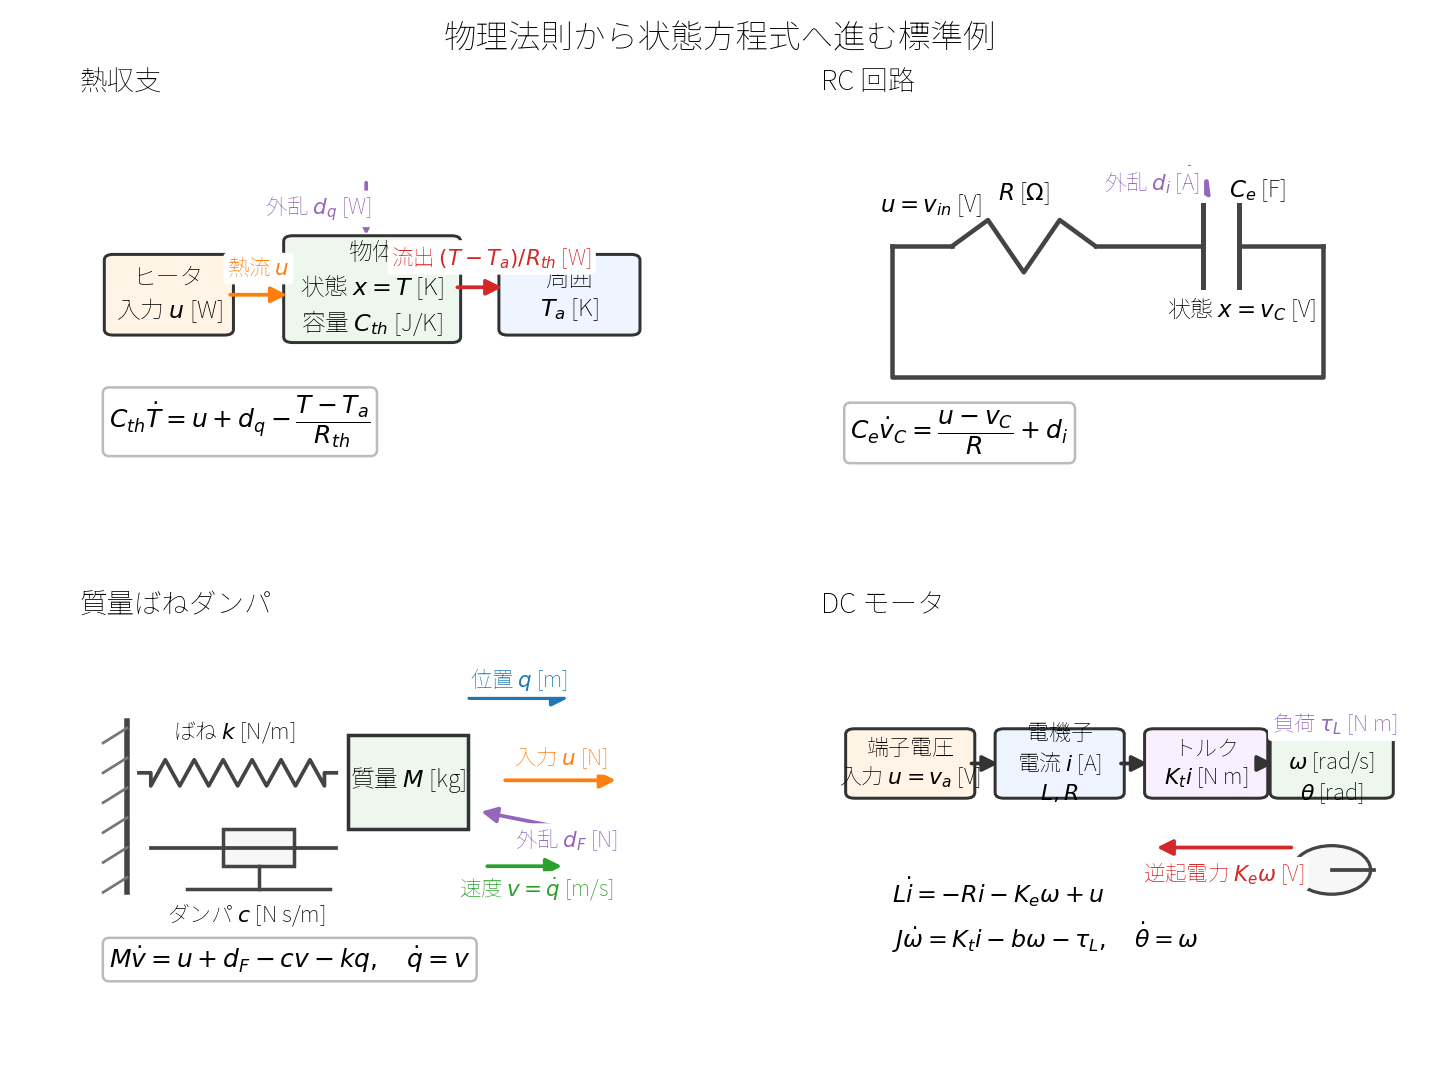
\includegraphics[width=0.96\linewidth,bb=0 0 1440 1080]{figures/physical_modeling_examples.png}
\caption{物理法則から状態方程式へ進む標準例。熱収支では内部エネルギーの蓄積、RC 回路では電荷の蓄積、質量ばねダンパ系では位置と速度、DC モータでは電流、角速度、角度を状態として残す。各パネルは入力、外乱、代表パラメータ、状態の単位を対応させ、保存則または運動方程式から $\dot{x}=f(x,u,d,p)$ へ整理する起点を示している。}
\label{fig:physical-modeling-examples}
\end{figure}

\begin{practice}[物理モデルの構造分類]
図\ref{fig:physical-modeling-examples} の四つの例について、蓄積される量、状態、入力、外乱、出力候補を一つずつ表にせよ。次に、熱系と RC 回路の式を見比べ、$C_{\mathrm{th}}$ と $C_e$、$R_{\mathrm{th}}$ と $R$、$T$ と $v_C$ がそれぞれどの役割に対応するかを説明せよ。最後に、質量ばねダンパ系で位置 $q$ だけを状態にした場合に未来の計算で不足する量を答えよ。
\end{practice}

\subsubsection{熱系の収支式からの導出}

一つの代表温度で表せる小さな物体を考える。温度を $T(t)$ [K]、周囲温度を $T_a(t)$ [K]、ヒータ熱流を $u(t)$ [W]、未知の熱流外乱を $d_q(t)$ [W] とする。熱容量を $C_{\mathrm{th}}$ [J/K]、熱抵抗を $R_{\mathrm{th}}$ [K/W] とし、物体内部の温度分布は無視できると仮定する。

蓄積される量は内部エネルギーであり、基準エネルギーを除けば変化率は
\begin{equation}
  \dot{E}(t)=C_{\mathrm{th}}\dot{T}(t)
\end{equation}
と書ける。単位は $(\mathrm{J/K})(\mathrm{K/s})=\mathrm{J/s}=\mathrm{W}$ であり、熱流と一致する。熱抵抗の構成則により、物体から周囲へ出る熱流は
\begin{equation}
  q_{\mathrm{out}}(t)=\frac{T(t)-T_a(t)}{R_{\mathrm{th}}}
\end{equation}
である。したがって熱収支は
\begin{align}
  C_{\mathrm{th}}\dot{T}(t)
  &=u(t)+d_q(t)-q_{\mathrm{out}}(t)\\
  &=u(t)+d_q(t)-\frac{T(t)-T_a(t)}{R_{\mathrm{th}}}
\end{align}
となる。状態を $x=T$、入力を $u$、外乱を
\begin{equation}
  d(t)=\begin{bmatrix}T_a(t)\\ d_q(t)\end{bmatrix}
\end{equation}
と選ぶと、一階の状態方程式は
\begin{equation}
  \dot{x}(t)
  =-\frac{1}{R_{\mathrm{th}}C_{\mathrm{th}}}x(t)
   +\frac{1}{C_{\mathrm{th}}}u(t)
   +\begin{bmatrix}
      \dfrac{1}{R_{\mathrm{th}}C_{\mathrm{th}}}&
      \dfrac{1}{C_{\mathrm{th}}}
    \end{bmatrix}d(t)
\end{equation}
である。出力として温度を測るなら
\begin{equation}
  y(t)=x(t)
\end{equation}
でよい。行列表示では $A=-1/(R_{\mathrm{th}}C_{\mathrm{th}})$、$B=1/C_{\mathrm{th}}$ であり、$A$ の単位は 1/s、$B$ の単位は K/J である。$B u$ の単位は $(\mathrm{K/J})(\mathrm{J/s})=\mathrm{K/s}$ となり、$\dot{x}$ の単位と一致する。

\subsubsection{RC 回路のキルヒホッフ則からの導出}

抵抗とコンデンサからなる一次の RC 回路を考える。入力電圧を $u(t)=v_{\mathrm{in}}(t)$ [V]、コンデンサ電圧を $v_C(t)$ [V]、節点へ流れ込む未知電流を $d_i(t)$ [A] とする。抵抗を $R$ [$\Omega$]、容量を $C_e$ [F] とし、抵抗と容量は一定、配線の寄生成分は無視できると仮定する。

蓄積される量はコンデンサの電荷
\begin{equation}
  Q_C(t)=C_e v_C(t)
\end{equation}
である。電荷の時間変化率は電流なので
\begin{equation}
  \dot{Q}_C(t)=C_e\dot{v}_C(t)
\end{equation}
であり、単位は $\mathrm{C/s}=\mathrm{A}$ である。抵抗を流れてコンデンサ節点へ入る電流は、オームの法則により
\begin{equation}
  i_R(t)=\frac{u(t)-v_C(t)}{R}
\end{equation}
である。キルヒホッフの電流則を節点に適用すると、コンデンサへ流れ込む電流の和が電荷の増加率になるため
\begin{align}
  C_e\dot{v}_C(t)&=i_R(t)+d_i(t)\\
  &=\frac{u(t)-v_C(t)}{R}+d_i(t)
\end{align}
を得る。状態を $x=v_C$、入力を $u=v_{\mathrm{in}}$、外乱を $d=d_i$ と置けば
\begin{align}
  \dot{x}(t)&=-\frac{1}{RC_e}x(t)+\frac{1}{RC_e}u(t)+\frac{1}{C_e}d(t),\\
  y(t)&=x(t)
\end{align}
である。このモデルでは $A=-1/(RC_e)$、$B=1/(RC_e)$ であり、どちらも 1/s の単位をもつ。電流外乱の係数 $1/C_e$ は、電流 [A] を電圧変化率 [V/s] に変える係数である。熱系と RC 回路の式が同じ形になるのは、熱容量とコンデンサ容量が蓄積を表し、熱抵抗と電気抵抗が差に比例する流れを作るからである。

\subsubsection{質量ばねダンパ系の運動方程式からの導出}

水平直線上の質量を考える。位置を $q(t)$ [m]、速度を $v(t)=\dot{q}(t)$ [m/s]、入力として加える力を $u(t)$ [N]、外力外乱を $d_F(t)$ [N] とする。質量を $M$ [kg]、粘性係数を $c$ [N\,s/m]、ばね定数を $k$ [N/m] とし、ばねの自然長からの変位を $q=0$ 基準で測る。

機械系では、力のつり合いではなくニュートンの第二法則を使う。運動量 $Mv$ の時間変化率が力の和であるから
\begin{equation}
  M\dot{v}(t)=\sum F(t)
\end{equation}
である。ばね力と粘性力の構成則を
\begin{equation}
  F_k(t)=-kq(t),\qquad F_c(t)=-cv(t)
\end{equation}
と置くと
\begin{align}
  M\dot{v}(t)&=u(t)+d_F(t)-cv(t)-kq(t),\\
  \dot{q}(t)&=v(t)
\end{align}
を得る。二階微分方程式としては
\begin{equation}
  M\ddot{q}(t)+c\dot{q}(t)+kq(t)=u(t)+d_F(t)
\end{equation}
であるが、状態方程式では一階の連立方程式に直す。状態を
\begin{equation}
  x(t)=\begin{bmatrix}q(t)\\ v(t)\end{bmatrix}
\end{equation}
と選ぶと
\begin{align}
  \dot{x}(t)
  &=\begin{bmatrix}
      0&1\\
      -k/M&-c/M
    \end{bmatrix}x(t)
    +\begin{bmatrix}
      0\\
      1/M
    \end{bmatrix}u(t)
    +\begin{bmatrix}
      0\\
      1/M
    \end{bmatrix}d_F(t),\label{eq:physical-modeling-msd-state}\\
  y(t)&=\begin{bmatrix}1&0\end{bmatrix}x(t)
\end{align}
となる。位置だけを測る場合は出力行列が $\begin{bmatrix}1&0\end{bmatrix}$ であり、速度まで測る場合は $y=x$ としてよい。\weq{physical-modeling-msd-state} の $A_{21}=-k/M$ は 1/s$^2$、$A_{22}=-c/M$ は 1/s、$B_2=1/M$ は 1/kg の単位をもつ。状態の成分 $q$ と $v$ の単位が異なるため、状態行列の各成分の単位も異なる。

熱系と RC 回路では一つの蓄積要素から一つの状態が生じた。質量ばねダンパ系では、位置だけでは次の位置を計算できず、速度も必要になる。したがって状態は $q$ だけでなく $v$ を含む。この違いは、モデルの次数が「式の見た目」ではなく、蓄積要素と将来計算に必要な情報の数で決まることを示している。

\subsubsection{DC モータの電気機械結合モデルの導出}

直流モータは、電気回路と回転運動が結合した標準的な制御対象である。ここでは電機子制御の DC モータを考え、端子電圧を $u(t)=v_a(t)$ [V]、電機子電流を $i(t)$ [A]、回転角を $\theta(t)$ [rad]、角速度を $\omega(t)=\dot{\theta}(t)$ [rad/s]、負荷トルクを $\tau_L(t)$ [N\,m] とする。電機子インダクタンスを $L$ [H]、電機子抵抗を $R$ [$\Omega$]、逆起電力定数を $K_e$ [V\,s/rad]、トルク定数を $K_t$ [N\,m/A]、回転部の等価慣性モーメントを $J$ [kg\,m$^2$]、粘性摩擦係数を $b$ [N\,m\,s/rad] とする。磁束は一定、磁気飽和、ブラシ電圧降下、クーロン摩擦、軸のねじれは無視し、すべてのパラメータは一定と仮定する。

電気側ではキルヒホッフの電圧則を使う。電機子端子に加えた電圧は、インダクタンスの電圧降下、抵抗の電圧降下、回転によって生じる逆起電力の和である。構成則を
\begin{equation}
  v_L(t)=L\dot{i}(t),\qquad
  v_R(t)=Ri(t),\qquad
  e_b(t)=K_e\omega(t)
\end{equation}
と置くと
\begin{equation}
  u(t)=L\dot{i}(t)+Ri(t)+K_e\omega(t)
\end{equation}
である。したがって電流の状態方程式は
\begin{equation}
  \dot{i}(t)=-\frac{R}{L}i(t)-\frac{K_e}{L}\omega(t)+\frac{1}{L}u(t)
  \label{eq:dcmotor-current-state}
\end{equation}
となる。各項の単位は A/s でそろう。たとえば $R i/L$ は V/H であり、$1\,\mathrm{H}=1\,\mathrm{V\,s/A}$ だから A/s である。

機械側では、回転に関するニュートンの第二法則を使う。角運動量 $J\omega$ の時間変化率は、軸まわりのトルクの和である。モータが作るトルクと粘性摩擦トルクを
\begin{equation}
  \tau_m(t)=K_t i(t),\qquad
  \tau_b(t)=b\omega(t)
\end{equation}
と置けば
\begin{equation}
  J\dot{\omega}(t)=K_t i(t)-b\omega(t)-\tau_L(t)
\end{equation}
であり、
\begin{equation}
  \dot{\omega}(t)=\frac{K_t}{J}i(t)-\frac{b}{J}\omega(t)-\frac{1}{J}\tau_L(t)
  \label{eq:dcmotor-speed-state}
\end{equation}
を得る。さらに角度は角速度の積分で決まるため
\begin{equation}
  \dot{\theta}(t)=\omega(t)
  \label{eq:dcmotor-angle-state}
\end{equation}
である。

角度制御まで含めるなら、状態を
\begin{equation}
  x(t)=\begin{bmatrix}i(t)\\ \omega(t)\\ \theta(t)\end{bmatrix},
  \qquad d(t)=\tau_L(t)
\end{equation}
と選ぶ。\weq{dcmotor-current-state}--\weq{dcmotor-angle-state} をまとめると
\begin{align}
  \dot{x}(t)
  &=
  \begin{bmatrix}
    -R/L&-K_e/L&0\\
    K_t/J&-b/J&0\\
    0&1&0
  \end{bmatrix}x(t)
  +\begin{bmatrix}
    1/L\\
    0\\
    0
  \end{bmatrix}u(t)
  +\begin{bmatrix}
    0\\
    -1/J\\
    0
  \end{bmatrix}d(t),\label{eq:dcmotor-state-space}\\
  y(t)&=C_y x(t)+D_y u(t)
\end{align}
となる。角速度を測って速度制御をする場合は $C_y=\begin{bmatrix}0&1&0\end{bmatrix}$、$D_y=0$ と置く。角度エンコーダで位置制御をする場合は $C_y=\begin{bmatrix}0&0&1\end{bmatrix}$ である。電流センサとエンコーダの両方を使うなら
\begin{equation}
  y(t)=
  \begin{bmatrix}
    1&0&0\\
    0&0&1
  \end{bmatrix}x(t)
\end{equation}
のように出力を複数にしてよい。

パラメータの意味は、応答の速さと結合の強さに直接現れる。$L/R$ は電気的時定数であり、回転が止まっていて逆起電力がないときの電流の立ち上がりを決める。$J/b$ は、電流を 0 として粘性摩擦だけで減速するときの機械的時定数である。$K_e$ が大きいほど同じ角速度で大きな逆起電力が生じ、電流の増加を抑える。$K_t$ が大きいほど同じ電流で大きなトルクが得られる。SI 単位系で同じ物理変換を理想的に表すと $K_t$ と $K_e$ の数値は一致するが、制御モデルでは単位と符号の定義を明示してから使う必要がある。負荷トルク $\tau_L$ は入力電圧で直接選べないため外乱として置き、速度低下や位置誤差を通じて観測される。

速度制御だけが目的で、角度 $\theta$ が出力にも制約にも入らない場合は、状態を $x=[i,\omega]^\T$ に縮約できる。一方、電気的時定数 $L/R$ が制御周期や機械応答に比べて十分小さい場合は、近似的に $L\dot{i}\simeq0$ と置き
\begin{equation}
  i(t)\simeq\frac{u(t)-K_e\omega(t)}{R}
\end{equation}
として、電流状態を消去する低次モデルを作ることもある。この近似は電流制御器が内側で十分速く働く場合にも使われる。ただし電流制限や過渡的なトルク応答を評価する設計では、\weq{dcmotor-state-space} のように電流を状態として残す方が適切である。

熱、電気、並進機械、回転機械の四例だけでは、保存則が流量で決まる対象と、重力で非線形な復元力を受ける対象をまだ十分に分けられない。水位制御では、センサが水位を測り、ポンプや弁が流量を変える。振子では、角度を測り、支点トルクで姿勢を変える。どちらも低次の制御対象として扱えるが、タンクでは流出量が水位の平方根に依存し、振子では重力項が $\sin\theta$ に依存する。図\ref{fig:tank-pendulum-modeling-examples} は、この二つの対象で、蓄積量、構成則、局所近似、パラメータ変化を対応させたものである。

\begin{figure}[tb]
\centering
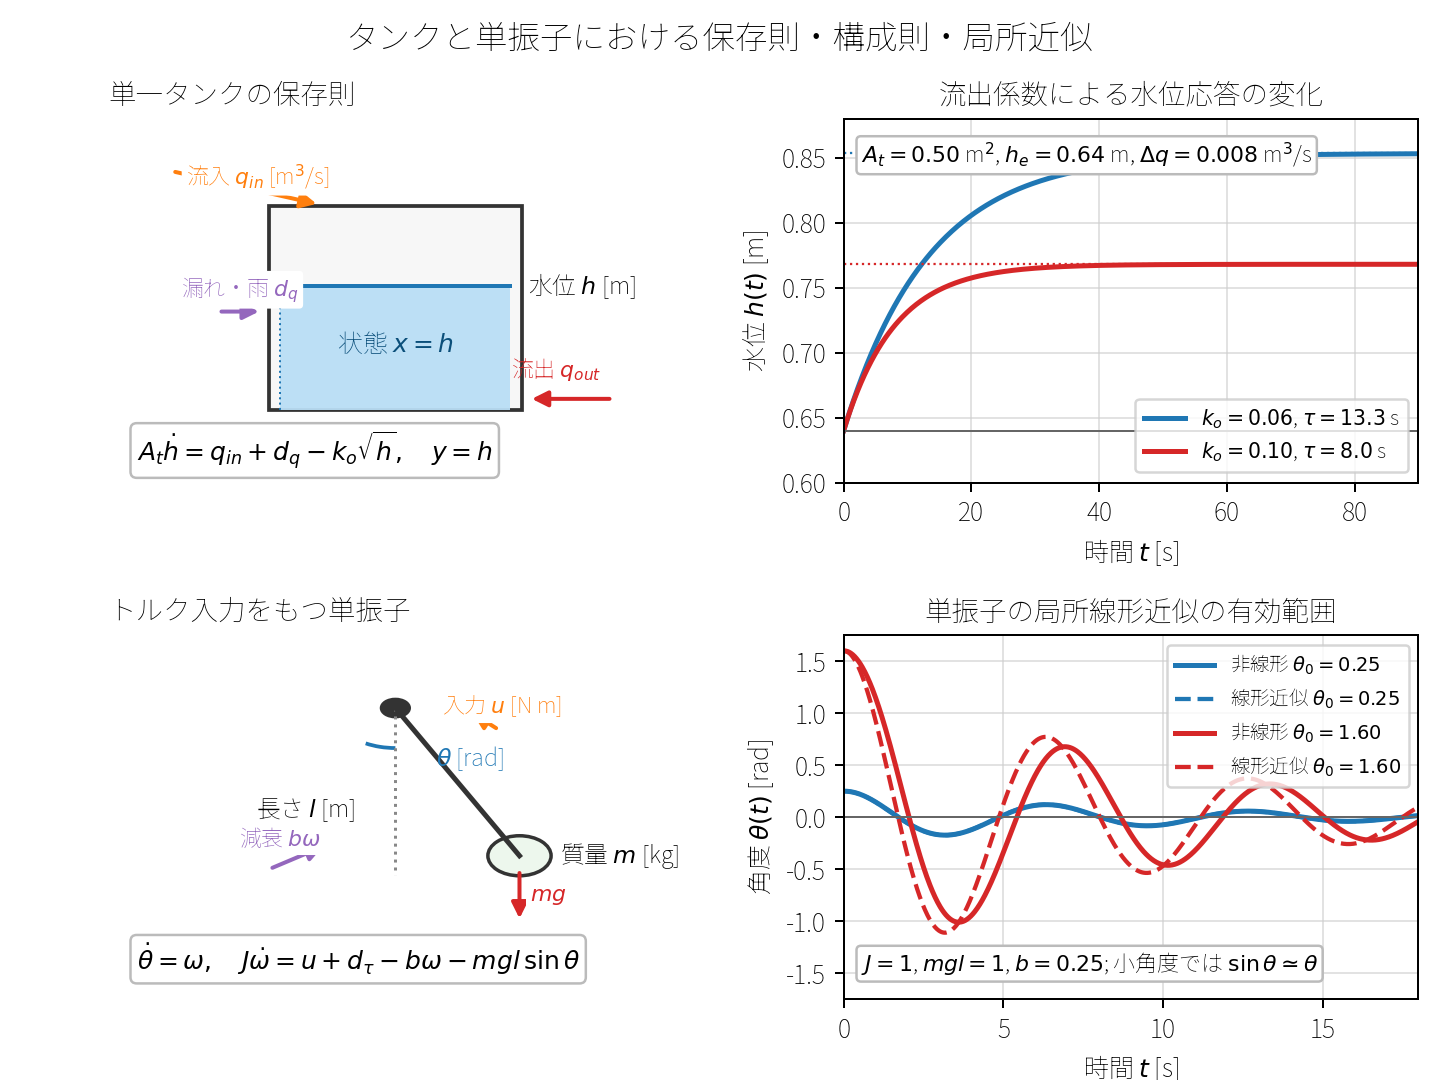
\includegraphics[width=0.96\linewidth,bb=0 0 1440 1080]{figures/tank_pendulum_modeling_examples.png}
\caption{タンク水位モデルと単振子モデルの構造。タンクでは体積保存則と流出構成則から水位の状態方程式が得られ、流出係数 $k_o$ を変えると線形化後の時定数と定常水位変化が同時に変わる。単振子ではトルク、重力、粘性減衰から角度と角速度の状態方程式が得られ、小角度では線形近似と非線形応答が一致しやすいが、大振幅では周期と振幅がずれる。}
\label{fig:tank-pendulum-modeling-examples}
\end{figure}

\subsubsection{単一タンクの水位状態方程式}

断面積が一定のタンクを考える。水位を $h(t)$ [m]、断面積を $A_t$ [m$^2$]、ポンプ流入を $q_{\mathrm{in}}(t)$ [m$^3$/s]、雨や漏れをまとめた流量外乱を $d_q(t)$ [m$^3$/s] とする。出力は水位センサで測る $y(t)=h(t)$ とする。タンク内の水量は体積
\begin{equation}
  V(t)=A_t h(t)
\end{equation}
であり、体積の時間変化率は流入から流出を引いた正味流量で決まる。

底の小さな出口から大気中へ流れる場合、流速は水位差によって変わる。ここでは出口断面積、流量係数、重力加速度をまとめた係数 $k_o$ を用いて
\begin{equation}
  q_{\mathrm{out}}(t)=k_o\sqrt{h(t)},\qquad h(t)\ge0
\end{equation}
と書く。$q_{\mathrm{out}}$ の単位は m$^3$/s なので、$k_o$ の単位は m$^{5/2}$/s である。したがって保存則は
\begin{align}
  \frac{\dd}{\dd t}\{A_t h(t)\}
  &=q_{\mathrm{in}}(t)+d_q(t)-q_{\mathrm{out}}(t)\\
  A_t\dot{h}(t)
  &=q_{\mathrm{in}}(t)+d_q(t)-k_o\sqrt{h(t)}
\end{align}
となる。状態を $x=h$ と選べば、非線形状態方程式は
\begin{align}
  \dot{x}(t)&=\frac{1}{A_t}\{q_{\mathrm{in}}(t)+d_q(t)-k_o\sqrt{x(t)}\},\label{eq:tank-level-state}\\
  y(t)&=x(t)
\end{align}
である。

一定流入 $q_{\mathrm{in},e}$ と一定外乱 $d_{q,e}$ のもとで水位 $h_e>0$ が保たれるには
\begin{equation}
  q_{\mathrm{in},e}+d_{q,e}=k_o\sqrt{h_e}
  \label{eq:tank-level-equilibrium}
\end{equation}
が必要である。この平衡点の近くで
\begin{equation}
  \tilde{h}=h-h_e,\qquad
  \tilde{q}_{\mathrm{in}}=q_{\mathrm{in}}-q_{\mathrm{in},e},\qquad
  \tilde{d}_q=d_q-d_{q,e}
\end{equation}
と置く。平方根を一次 Taylor 展開すると
\begin{equation}
  \sqrt{h_e+\tilde{h}}
  =\sqrt{h_e}+\frac{1}{2\sqrt{h_e}}\tilde{h}
  +O(\tilde{h}^2)
\end{equation}
である。\weq{tank-level-equilibrium} を使って定数項を消すと、一次近似は
\begin{equation}
  A_t\dot{\tilde{h}}
  =\tilde{q}_{\mathrm{in}}+\tilde{d}_q
  -\frac{k_o}{2\sqrt{h_e}}\tilde{h}
\end{equation}
となる。したがって
\begin{equation}
  \dot{\tilde{h}}
  =-\frac{k_o}{2A_t\sqrt{h_e}}\tilde{h}
   +\frac{1}{A_t}\tilde{q}_{\mathrm{in}}
   +\frac{1}{A_t}\tilde{d}_q
  \label{eq:tank-level-linearization}
\end{equation}
である。流出係数 $k_o$ が大きいほど、水位のずれを戻す係数 $k_o/(2A_t\sqrt{h_e})$ は大きくなり、時定数
\begin{equation}
  \tau_h=\frac{2A_t\sqrt{h_e}}{k_o}
\end{equation}
は短くなる。一方、同じ流入増分 $\Delta q$ に対する定常水位増分は
\begin{equation}
  \Delta h_\infty=\frac{2\sqrt{h_e}}{k_o}\Delta q
\end{equation}
であり、$k_o$ が大きいほど小さい。図\ref{fig:tank-pendulum-modeling-examples} の右上は、この二つの効果を同じ線形化モデルで示している。

\subsubsection{単振子のトルク入力状態方程式}

長さ $l$ [m] の軽い棒の先に質量 $m$ [kg] があり、支点まわりにトルク入力 $u(t)$ [N\,m] を加えられる単振子を考える。角度 $\theta(t)$ [rad] は下向きから測り、角速度を $\omega(t)=\dot{\theta}(t)$ [rad/s] とする。支点の粘性減衰係数を $b$ [N\,m\,s/rad]、外乱トルクを $d_\tau(t)$ [N\,m] とし、棒の質量と支点の摩擦以外の損失は無視する。質点モデルでは支点まわりの慣性モーメントは
\begin{equation}
  J=ml^2
\end{equation}
である。

角運動量 $J\omega$ の時間変化率は、支点まわりのトルクの和で決まる。入力トルクと外乱トルクは正方向へ入り、粘性減衰は $-b\omega$、重力の復元トルクは $-mgl\sin\theta$ である。したがって
\begin{equation}
  J\dot{\omega}(t)
  =u(t)+d_\tau(t)-b\omega(t)-mgl\sin\theta(t)
\end{equation}
であり、状態を
\begin{equation}
  x(t)=\begin{bmatrix}\theta(t)\\ \omega(t)\end{bmatrix}
\end{equation}
と置くと
\begin{align}
  \dot{x}_1(t)&=x_2(t),\\
  \dot{x}_2(t)&=\frac{1}{J}\{u(t)+d_\tau(t)-b x_2(t)-mgl\sin x_1(t)\},\label{eq:pendulum-state}\\
  y(t)&=x_1(t)
\end{align}
を得る。

角度 $\theta_e$ で静止させたいとき、$\omega_e=0$ として平衡入力は
\begin{equation}
  u_e=mgl\sin\theta_e-d_{\tau,e}
\end{equation}
である。偏差を $\tilde{\theta}=\theta-\theta_e$、$\tilde{\omega}=\omega$、$\tilde{u}=u-u_e$、$\tilde{d}_\tau=d_\tau-d_{\tau,e}$ と置き、$\sin(\theta_e+\tilde{\theta})$ を一次 Taylor 展開すると
\begin{equation}
  \sin(\theta_e+\tilde{\theta})
  =\sin\theta_e+\cos\theta_e\,\tilde{\theta}+O(\tilde{\theta}^2)
\end{equation}
である。定数項は平衡条件で消えるので、接線モデルは
\begin{equation}
  \begin{bmatrix}
    \dot{\tilde{\theta}}\\
    \dot{\tilde{\omega}}
  \end{bmatrix}
  =
  \begin{bmatrix}
    0&1\\
    -mgl\cos\theta_e/J&-b/J
  \end{bmatrix}
  \begin{bmatrix}
    \tilde{\theta}\\
    \tilde{\omega}
  \end{bmatrix}
  +\begin{bmatrix}0\\1/J\end{bmatrix}\tilde{u}
  +\begin{bmatrix}0\\1/J\end{bmatrix}\tilde{d}_\tau .
  \label{eq:pendulum-linearization}
\end{equation}
下向き平衡点 $\theta_e=0$ では $\cos\theta_e=1$ なので重力項は復元力として働く。上向き平衡点 $\theta_e=\pi$ では $\cos\theta_e=-1$ なので符号が反転し、角度のずれをさらに大きくする不安定化項になる。同じ振子でも、平衡点をどこに選ぶかにより線形化モデルの安定性が変わる。

図\ref{fig:tank-pendulum-modeling-examples} の右下では、$J=1$、$mgl=1$、$b=0.25$ として下向き平衡点まわりの自由応答を比べている。初期角度が $0.25\,\mathrm{rad}$ 程度なら $\sin\theta\simeq\theta$ による線形近似は非線形応答とよく合う。一方、初期角度が $1.60\,\mathrm{rad}$ まで大きくなると、復元トルクが角度に比例しなくなり、振動周期と振幅の減衰が線形近似からずれる。この差は、線形化が「対象を単純にする公式」ではなく、平衡点近くの局所モデルであることを示している。

\begin{practice}[タンクと単振子の状態選択]
図\ref{fig:tank-pendulum-modeling-examples} のタンクについて、$A_t=0.50\,\mathrm{m^2}$、$h_e=0.64\,\mathrm{m}$、$k_o=0.10\,\mathrm{m^{5/2}/s}$ のとき、外乱が 0 なら平衡流入 $q_{\mathrm{in},e}$ はいくらか計算せよ。次に \weq{tank-level-linearization} の係数 $k_o/(2A_t\sqrt{h_e})$ と時定数 $\tau_h$ を求め、$k_o=0.06\,\mathrm{m^{5/2}/s}$ の場合と比べよ。単振子については、\weq{pendulum-linearization} で $\theta_e=0$ と $\theta_e=\pi$ を代入し、重力項の符号が変わる理由を、下向き平衡点と上向き平衡点の小さなずれに対応させて説明せよ。
\end{practice}

\subsubsection{台車上倒立振子の非線形モデルと線形化}

倒立振子は、非線形性、不安定平衡点、状態選択、線形化の意味を同時に示す標準例である。ここでは水平に動く台車の上に剛体棒を取り付けた系を、棒の重心に質量が集中したモデルとして導く。台車位置を $q(t)$ [m]、台車速度を $v(t)=\dot{q}(t)$ [m/s]、振子角を $\theta(t)$ [rad]、角速度を $\omega(t)=\dot{\theta}(t)$ [rad/s] とする。角度 $\theta=0$ は直立上向きであり、$\theta>0$ は重心が右へ傾く向きとする。台車質量を $M$ [kg]、振子質量を $m$ [kg]、支点から重心までの距離を $l$ [m]、重力加速度を $g$ [m/s$^2$]、台車へ加える水平力を $u(t)$ [N] とする。車輪や支点の摩擦、棒の慣性、アクチュエータの飽和はまず無視する。

振子重心の座標を、上向きを正の鉛直方向として
\begin{equation}
  X(t)=q(t)+l\sin\theta(t),\qquad
  Y(t)=l\cos\theta(t)
\end{equation}
と書く。速度は
\begin{equation}
  \dot{X}=\dot{q}+l\cos\theta\,\dot{\theta},
  \qquad
  \dot{Y}=-l\sin\theta\,\dot{\theta}
\end{equation}
である。運動エネルギー $T$ と位置エネルギー $V$ は
\begin{align}
  T&=\frac{1}{2}M\dot{q}^2
    +\frac{1}{2}m(\dot{X}^2+\dot{Y}^2)\\
   &=\frac{1}{2}(M+m)\dot{q}^2
    +m l\cos\theta\,\dot{q}\dot{\theta}
    +\frac{1}{2}m l^2\dot{\theta}^2,\\
  V&=m g l\cos\theta
\end{align}
である。一般化座標を $q$ と $\theta$ とし、ラグランジアンを $\mathcal{L}=T-V$ とする。台車方向の一般化力は $Q_q=u$、角度方向の一般化力は $Q_\theta=0$ である。

オイラー・ラグランジュ方程式
\begin{equation}
  \frac{\dd}{\dd t}\frac{\pp \mathcal{L}}{\pp \dot{q}_j}
  -\frac{\pp \mathcal{L}}{\pp q_j}=Q_j
\end{equation}
を $q$ に適用する。まず
\begin{equation}
  \frac{\pp \mathcal{L}}{\pp \dot{q}}
  =(M+m)\dot{q}+m l\cos\theta\,\dot{\theta}
\end{equation}
であり、
\begin{equation}
  \frac{\dd}{\dd t}\frac{\pp \mathcal{L}}{\pp \dot{q}}
  =(M+m)\ddot{q}+m l\cos\theta\,\ddot{\theta}
  -m l\sin\theta\,\dot{\theta}^2
\end{equation}
となる。$\mathcal{L}$ は $q$ に陽に依存しないので $\pp\mathcal{L}/\pp q=0$ である。したがって
\begin{equation}
  (M+m)\ddot{q}+m l\cos\theta\,\ddot{\theta}
  -m l\sin\theta\,\dot{\theta}^2=u
  \label{eq:cartpole-q-equation}
\end{equation}
を得る。

同じ式を $\theta$ に適用する。偏微分は
\begin{align}
  \frac{\pp \mathcal{L}}{\pp \dot{\theta}}
  &=m l\cos\theta\,\dot{q}+m l^2\dot{\theta},\\
  \frac{\dd}{\dd t}\frac{\pp \mathcal{L}}{\pp \dot{\theta}}
  &=m l\cos\theta\,\ddot{q}
    -m l\sin\theta\,\dot{\theta}\dot{q}
    +m l^2\ddot{\theta},\\
  \frac{\pp \mathcal{L}}{\pp \theta}
  &=-m l\sin\theta\,\dot{q}\dot{\theta}
    +m g l\sin\theta
\end{align}
である。これを差し引くと速度積の項が消え、
\begin{equation}
  m l\cos\theta\,\ddot{q}+m l^2\ddot{\theta}
  -m g l\sin\theta=0
  \label{eq:cartpole-theta-equation}
\end{equation}
となる。\weq{cartpole-q-equation} と \weq{cartpole-theta-equation} を加速度についてまとめると
\begin{equation}
  \begin{bmatrix}
    M+m&m l\cos\theta\\
    m l\cos\theta&m l^2
  \end{bmatrix}
  \begin{bmatrix}
    \ddot{q}\\
    \ddot{\theta}
  \end{bmatrix}
  =
  \begin{bmatrix}
    u+m l\sin\theta\,\dot{\theta}^2\\
    m g l\sin\theta
  \end{bmatrix}.
  \label{eq:cartpole-mass-matrix}
\end{equation}
左辺の行列は、一般化座標に対応する慣性行列である。行列式は
\begin{equation}
  \Delta(\theta)=m l^2\{M+m\sin^2\theta\}
\end{equation}
であり、$M>0$、$m>0$、$l>0$ なら常に正である。したがって加速度を一意に解ける。

状態を
\begin{equation}
  x(t)=\begin{bmatrix}q(t)\\ v(t)\\ \theta(t)\\ \omega(t)\end{bmatrix}
\end{equation}
と置き、$v=\dot{q}$、$\omega=\dot{\theta}$ を使うと、非線形状態方程式は
\begin{align}
  \dot{x}_1&=x_2,\\
  \dot{x}_2&=
  \frac{u+m l x_4^2\sin x_3-m g\sin x_3\cos x_3}
       {M+m\sin^2 x_3},\label{eq:cartpole-nonlinear-qddot}\\
  \dot{x}_3&=x_4,\\
  \dot{x}_4&=
  \frac{(M+m)g\sin x_3-\cos x_3\{u+m l x_4^2\sin x_3\}}
       {l\{M+m\sin^2 x_3\}}.
  \label{eq:cartpole-nonlinear-thetaddot}
\end{align}
台車位置と振子角を測るなら、出力方程式は
\begin{equation}
  y(t)=
  \begin{bmatrix}
    1&0&0&0\\
    0&0&1&0
  \end{bmatrix}x(t)
\end{equation}
である。速度センサがない場合でも $v$ と $\omega$ は未来を決めるために状態に含める。測定されない速度は、数値微分、オブザーバ、または推定器で補う対象になる。

直立平衡点は、任意の一定位置 $q_e$ に対して
\begin{equation}
  x_e=\begin{bmatrix}q_e\\ 0\\ 0\\ 0\end{bmatrix},
  \qquad u_e=0
\end{equation}
である。直立近傍で $\sin\theta\simeq\theta$、$\cos\theta\simeq1$、$\theta^2$ と $\omega^2\theta$ を二次以上の小さい項として捨てると
\begin{align}
  \ddot{q}&\simeq \frac{1}{M}u-\frac{m g}{M}\theta,\\
  \ddot{\theta}&\simeq -\frac{1}{lM}u+\frac{(M+m)g}{lM}\theta
\end{align}
である。したがって偏差状態 $\tilde{x}=[\tilde{q},\tilde{v},\tilde{\theta},\tilde{\omega}]^\T$ は
\begin{equation}
  \dot{\tilde{x}}=
  \begin{bmatrix}
    0&1&0&0\\
    0&0&-m g/M&0\\
    0&0&0&1\\
    0&0&(M+m)g/(lM)&0
  \end{bmatrix}\tilde{x}
  +\begin{bmatrix}
    0\\
    1/M\\
    0\\
    -1/(lM)
  \end{bmatrix}\tilde{u}
  \label{eq:cartpole-linearized-upright}
\end{equation}
に従う。$A_{43}=(M+m)g/(lM)$ が正であるため、角度がわずかに正へ傾くと角加速度も正になり、開ループでは直立平衡点から離れる。これが倒立振子の不安定性である。台車入力 $\tilde{u}$ は、台車加速度を直接作ると同時に、支点加速度を通じて角加速度へ反対符号で入る。

$M$ は入力力から台車加速度への変換を弱める等価質量であり、大きいほど同じ力で動きにくい。$m$ は重力による倒れ込みと台車への反作用を強くする。$l$ が長いほど、同じ支点加速度による角加速度は小さくなり、重力による角加速度の係数も $1/l$ に比例して小さくなる。棒の重心まわりの慣性モーメントを無視できない場合は、$m l^2$ を支点まわりの慣性モーメント $I_p$ に置き換えて同じ手順を使う。実機では台車摩擦 $c$ [N\,s/m] や支点摩擦 $b_p$ [N\,m\,s/rad] を無視できないこともある。その場合は \weq{cartpole-mass-matrix} の右辺第一成分に $-c\dot{q}$、第二成分に $-b_p\dot{\theta}$ を追加してから状態方程式と線形化を作ればよい。

\subsection{入出力微分方程式と状態空間実現の対応}

物理法則から得たモデルは、内部の蓄積量を状態として残すと状態空間モデルになる。一方、外から加える入力 $u$ と外へ取り出す出力 $y$ だけに注目すると、内部状態を消去した入出力微分方程式としても書ける。両者は別の対象を表しているのではなく、同じ線形時不変モデルを異なる座標と情報量で表したものである。

\subsubsection{入出力微分方程式の標準形}

一入力一出力の線形時不変モデルでは、定数係数の入出力微分方程式を
\begin{equation}
  a_n y^{(n)}(t)+a_{n-1}y^{(n-1)}(t)+\cdots+a_1\dot{y}(t)+a_0y(t)
  =
  b_m u^{(m)}(t)+b_{m-1}u^{(m-1)}(t)+\cdots+b_1\dot{u}(t)+b_0u(t)
  \label{eq:iomodel-differential-form}
\end{equation}
と書く。ここで $a_n\ne0$、$y^{(i)}=\dd^i y/\dd t^i$、$u^{(i)}=\dd^i u/\dd t^i$ である。通常の有限次元状態空間モデルから入力を微分せずに作られる伝達関数はプロパーなので、入力側の最高階数は $m\le n$ である。$m=n$ の項は入力が出力へ状態を経ずに同時に現れる直達項に対応し、$m<n$ なら直達項をもたない。

\weq{iomodel-differential-form} は、入力と出力の関係を直接表すため、実験データからモデル次数や係数を同定するときに扱いやすい。しかし、初期温度、コンデンサ電圧、速度のような内部に蓄えられた情報は、出力とその微分の初期値として間接的にしか現れない。状態空間モデルは、この内部情報を状態ベクトルとして明示する表現である。

\begin{definition}[実現]
伝達関数または入出力微分方程式と同じ零初期状態の入出力関係をもつ状態空間モデル
\begin{align}
  \dot{x}(t)&=Ax(t)+Bu(t),\\
  y(t)&=Cx(t)+Du(t)
\end{align}
を、その入出力モデルの実現という。
\end{definition}

分母をモニックに正規化したプロパーな伝達関数を
\begin{equation}
  G(s)=D+\frac{\bar{b}_{n-1}s^{n-1}+\bar{b}_{n-2}s^{n-2}+\cdots+\bar{b}_1s+\bar{b}_0}
  {s^n+a_{n-1}s^{n-1}+\cdots+a_1s+a_0}
  \label{eq:proper-transfer-realization-source}
\end{equation}
と書く。このとき一つの実現は
\begin{align}
  \dot{x}(t)
  &=
  \begin{bmatrix}
    0&1&0&\cdots&0\\
    0&0&1&\cdots&0\\
    \vdots&\vdots&\vdots&\ddots&\vdots\\
    0&0&0&\cdots&1\\
    -a_0&-a_1&-a_2&\cdots&-a_{n-1}
  \end{bmatrix}x(t)
  +\begin{bmatrix}
    0\\
    0\\
    \vdots\\
    0\\
    1
  \end{bmatrix}u(t),\label{eq:controllable-canonical-realization}\\
  y(t)&=
  \begin{bmatrix}
    \bar{b}_0&\bar{b}_1&\bar{b}_2&\cdots&\bar{b}_{n-1}
  \end{bmatrix}x(t)+Du(t)
\end{align}
である。この形を可制御正準形という。状態の成分は、必ずしも温度、電圧、位置のような物理量そのものではない。入出力関係を再現するために作った内部座標であり、物理法則から選んだ状態とは異なる単位や意味をもつことがある。

\subsubsection{状態方程式から伝達関数への導出}

連続時間の線形時不変状態方程式
\begin{align}
  \dot{x}(t)&=Ax(t)+Bu(t),\label{eq:ss-to-tf-state}\\
  y(t)&=Cx(t)+Du(t)\label{eq:ss-to-tf-output}
\end{align}
を考える。$x\in\R^n$、$u\in\R^m$、$y\in\R^p$ とし、$A,B,C,D$ は定数行列である。$D$ は直達行列であり、入力が状態の積分を待たずに出力へ現れる成分を表す。

\begin{derivation}
\weq{ss-to-tf-state} をラプラス変換する。$X(s)$、$U(s)$、$Y(s)$ をそれぞれ $x(t)$、$u(t)$、$y(t)$ のラプラス変換とすると、微分公式より
\begin{equation}
  sX(s)-x(0)=AX(s)+BU(s)
\end{equation}
である。これを $X(s)$ について解くと
\begin{align}
  (sI-A)X(s)&=x(0)+BU(s),\\
  X(s)&=(sI-A)^{-1}x(0)+(sI-A)^{-1}BU(s)
\end{align}
を得る。ただし、$sI-A$ が正則な $s$ を考える。出力方程式のラプラス変換は
\begin{equation}
  Y(s)=CX(s)+DU(s)
\end{equation}
であるから、
\begin{equation}
  Y(s)=C(sI-A)^{-1}x(0)+\{C(sI-A)^{-1}B+D\}U(s)
  \label{eq:ss-laplace-with-initial}
\end{equation}
となる。零初期状態 $x(0)=0$ では、入力から出力への伝達関数行列は
\begin{equation}
  G(s)=C(sI-A)^{-1}B+D
  \label{eq:ss-transfer-function}
\end{equation}
である。
\end{derivation}

\weq{ss-laplace-with-initial} の第一項は、入力とは独立に初期状態から生じる自然応答である。したがって伝達関数 $G(s)$ は「初期状態を 0 にそろえたとき、入力が出力へどう伝わるか」を表す。初期状態が 0 でなければ、同じ入力を加えても出力は変わる。実験で伝達関数を測るときに、対象を十分静止させる、コンデンサを放電する、温度を基準値へ戻す、といった操作を行うのは、初期状態による応答を入力応答から分けるためである。

\subsubsection{最小実現と非最小実現}

同じ伝達関数を表す状態空間モデルは一つではない。正則行列 $T$ を用いて座標変換 $x=Tz$ を行うと
\begin{align}
  \dot{z}(t)&=T^{-1}ATz(t)+T^{-1}Bu(t),\\
  y(t)&=CTz(t)+Du(t)
\end{align}
となるが、伝達関数は
\begin{equation}
  CT\{sI-T^{-1}AT\}^{-1}T^{-1}B+D
  =
  C(sI-A)^{-1}B+D
\end{equation}
のまま変わらない。これは、状態座標の選び方が変わっても零初期状態の入出力関係は同じであることを示している。

さらに、入出力に全く現れない余分な状態を追加しても、伝達関数は変わらない。たとえば
\begin{align}
  \dot{x}_1&=-x_1+u,\\
  \dot{x}_2&=-5x_2,\\
  y&=x_1
\end{align}
では、$x_2$ は入力からも出力からも切り離されている。零初期状態の伝達関数は
\begin{equation}
  G(s)=\frac{1}{s+1}
\end{equation}
であり、$x_2$ に対応する固有値 $-5$ は伝達関数の極として現れない。このように余分な状態を含む実現を非最小実現という。これに対して、入力から動かせる状態だけをもち、かつ出力から区別できる状態だけをもつ実現を最小実現という。最小実現の次数は、極零相殺を除いた伝達関数の分母次数と一致する。可制御性と可観測性を用いた厳密な判定は、後の状態空間制御の章で扱う。

\subsubsection{極と零点の初等的解釈}

一入力一出力のプロパーな伝達関数を
\begin{equation}
  G(s)=\frac{N(s)}{P(s)}
\end{equation}
と書く。共通因子を約分した後の分母 $P(s)$ の根を極、分子 $N(s)$ の根を零点という。極は、零入力でも残る自然応答の指数関数 $e^{pt}$ の指数 $p$ に対応する。実部が負ならそのモードは減衰し、実部が正なら増大する。状態行列 $A$ の固有値は内部モードの候補であるが、非最小実現では入力から動かせない、または出力に現れない固有値が伝達関数の極から消えることがある。

零点は、入力によって作られる複数の経路が出力で打ち消し合う複素数である。$s=z$ で $N(z)=0$ なら、形式的には $e^{zt}$ 型の入力成分に対する零初期状態の出力が打ち消される。零点は応答の立ち上がり、逆応答、制御器で無理に打ち消してよいかどうかに関わる。極が主に自然な時間スケールを表すのに対し、零点は入力から出力へ至る経路の符号と相対的な速さを表す量として解釈できる。

\subsubsection{質量ばねダンパ系の双方向変換例}

質量ばねダンパ系
\begin{equation}
  M\ddot{q}(t)+c\dot{q}(t)+kq(t)=u(t),
  \qquad y(t)=q(t)
  \label{eq:msd-io-for-realization}
\end{equation}
を考える。$M>0$、$c\ge0$、$k>0$ とし、入力 $u$ の単位は N、出力 $y$ の単位は m である。物理状態を
\begin{equation}
  x(t)=\begin{bmatrix}q(t)\\ \dot{q}(t)\end{bmatrix}
\end{equation}
と選ぶと
\begin{align}
  \dot{x}(t)&=
  \begin{bmatrix}
    0&1\\
    -k/M&-c/M
  \end{bmatrix}x(t)
  +\begin{bmatrix}
    0\\
    1/M
  \end{bmatrix}u(t),\\
  y(t)&=\begin{bmatrix}1&0\end{bmatrix}x(t)
  \label{eq:msd-physical-realization}
\end{align}
となる。この状態空間モデルから伝達関数を計算する。ここでは
\begin{equation}
  sI-A=
  \begin{bmatrix}
    s&-1\\
    k/M&s+c/M
  \end{bmatrix}
\end{equation}
であり、行列式は
\begin{equation}
  \det(sI-A)=s^2+\frac{c}{M}s+\frac{k}{M}
\end{equation}
である。したがって
\begin{align}
  (sI-A)^{-1}B
  &=
  \frac{1}{s^2+(c/M)s+k/M}
  \begin{bmatrix}
    s+c/M&1\\
    -k/M&s
  \end{bmatrix}
  \begin{bmatrix}
    0\\
    1/M
  \end{bmatrix}\\
  &=
  \frac{1}{s^2+(c/M)s+k/M}
  \begin{bmatrix}
    1/M\\
    s/M
  \end{bmatrix}.
\end{align}
$C=\begin{bmatrix}1&0\end{bmatrix}$、$D=0$ なので
\begin{equation}
  G(s)=C(sI-A)^{-1}B
  =
  \frac{1/M}{s^2+(c/M)s+k/M}
  =
  \frac{1}{Ms^2+cs+k}
  \label{eq:msd-transfer-from-state}
\end{equation}
を得る。

逆に、伝達関数 \weq{msd-transfer-from-state} から入出力微分方程式へ戻す。零初期状態では
\begin{equation}
  (Ms^2+cs+k)Y(s)=U(s)
\end{equation}
である。ラプラス変換の微分公式を時間領域へ戻すと
\begin{equation}
  M\ddot{y}(t)+c\dot{y}(t)+ky(t)=u(t)
\end{equation}
であり、$y=q$ と置けば \weq{msd-io-for-realization} と一致する。同じ伝達関数を可制御正準形で実現するなら
\begin{align}
  \dot{z}(t)&=
  \begin{bmatrix}
    0&1\\
    -k/M&-c/M
  \end{bmatrix}z(t)
  +\begin{bmatrix}
    0\\
    1
  \end{bmatrix}u(t),\\
  y(t)&=\begin{bmatrix}1/M&0\end{bmatrix}z(t)
\end{align}
としてもよい。この $z$ は物理状態 $[q,\dot{q}]^\T$ ではないが、零初期状態の入力 $u$ から出力 $y$ への関係は同じである。物理的解釈を重視するときは $x=[q,\dot{q}]^\T$ が自然であり、係数比較や設計計算を整理したいときは正準形が便利である。
